\documentclass[USenglish]{tex/lipics-v2016}
\usepackage{stmaryrd} 
\usepackage{xspace,listings,url,framed,amssymb,
            hyperref,doi, mathtools,wrapfig,
            stmaryrd, graphicx, tikz, colortbl, xparse, etoolbox,
            pgffor, makecell, microtype}
            \usetikzlibrary{decorations.pathreplacing}

\usepackage[customcolors,norndcorners]{hf-tikz}
\usepackage{tex/mathpartir}
\usetikzlibrary{arrows}
\usetikzlibrary{shapes.geometric}
\usetikzlibrary{shapes.multipart}
\usetikzlibrary{positioning}
\usetikzlibrary{calc}
\usetikzlibrary{backgrounds}
\usepackage[inline]{enumitem}
\usepackage{epigraph}
\setlength{\epigraphrule}{0pt}
\renewcommand*{\textflush}{flushright}
\setlength{\epigraphwidth}{4in}
\newcommand{\code}[1]{{\tt #1}\xspace}
\newcommand{\FZ}[1]{\textbf{FZ: #1}}
%% Formatting
\newcommand{\EM}[1]{\ensuremath{#1}\xspace}
\newcommand{\xt}[1]{{\sf{#1}}}
\newcommand{\bt}[1]{\xt{\bf #1}}
\renewcommand{\b}[1]{\EM{\overline{#1}}}
\newcommand{\EMxt}[1]{\EM{\xt{#1}}}
\newcommand{\EMbt}[1]{\EM{\bt{#1}}}

%% Variables
\newcommand{\x}   {\EMxt x}
\newcommand{\n}   {\EMxt n}
\newcommand{\e}   {\EMxt e}
\newcommand{\m}   {\EMxt m}
\newcommand{\s}   {\EM{\sigma}}
\renewcommand{\t} {\EMxt t}
\newcommand{\ta}  {\EM{\tau}}
\renewcommand{\a} {\EMxt a}
\newcommand{\K}   {\EMxt K}
\renewcommand{\k} {\EMxt k}
\newcommand{\Kp}  {{\EMxt{K'}}}
\newcommand{\Kpp}  {{\EMxt{K''}}}
\newcommand{\Kppp}  {{\EMxt{K'''}}}
\newcommand{\ep}  {{{\EMxt{e'}}}}
\newcommand{\epp}  {{{\EMxt{e''}}}}
\renewcommand{\sp}{{{\EM{\s'}}}}
\newcommand{\spp}{{{\EM{\s''}}}}
\newcommand{\ap}  {\EM{\a'}}
\newcommand{\aE}[1]  {\EM{\a_{#1}}}
\newcommand{\app}  {\EM{\a''}}
\newcommand{\tp}  {\EM{ \t'}}
\newcommand{\tpp}  {\EM{ \t''}}
\newcommand{\C}   {\EMxt C}
\newcommand{\Cp}  {\EMxt{C'}}
\newcommand{\EC}   {\EMxt E}
\newcommand{\fd}  {\EMxt{fd}}
\newcommand{\md}  {\EMxt{md}}
\newcommand{\mdpp}  {\EM{\md'}}
\newcommand{\mt}  {\EMxt{mt}}
\newcommand{\mtp}  {\EMxt{mt'}}
\newcommand{\mtpp}  {\EMxt{mt''}}
\newcommand{\M}{\EMxt M}
\newcommand{\MN}  {\EMxt{M\,K}}
\newcommand{\MNargs}[1]  {\EMxt {M #1~K}}
\newcommand{\f}   {\EMxt f}
\newcommand{\fp}   {\EMxt{ f'}}
\newcommand{\E}   {\EM{\Gamma}}
\newcommand{\EE}   {\EM{\mathcal{E}}}
\newcommand{\any} {\EM{\star}}
\newcommand{\this}{\EMxt{this}}
\newcommand{\that}{\EMxt{that}}
\newcommand{\none}{\EM{\cdot}}
\newcommand{\D}   {\EMxt D}
\newcommand{\Dp}   {\EMxt{D'}}
\newcommand{\p}   {\EMxt p}
\newcommand{\np}{\n'}

\newcommand{\Get}[2]   {\EM{#1.#2()}}
\newcommand{\Set}[3]   {\EM{#1.#2(#3)}}
\newcommand{\Call}[3]  {\EM{#1.#2(#3)}}
\newcommand{\DynCall}[3]  {\EM{#1@#2(#3)}}

\newcommand{\New}[2]   {\EM{\new\;#1(#2)}}
\newcommand{\SubCast}[2]{\EM{<\hspace{-.6mm}{#1}\hspace{-.6mm}>\hspace{-1mm}\;{#2}}}
\newcommand{\ShaCast}[2]{\EM{\prec #1 \succ #2}}
\newcommand{\MonCast}[2]{\EM{\triangleleft\; #1 \triangleright #2}}
\newcommand{\BehCast}[2]{\EM{\blacktriangleleft #1 \blacktriangleright #2}}
\newcommand{\new}      {\EM{\bt{new}}}
\newcommand{\HT}[2]    {\EM{{#1}\!:{#2}}}
\newcommand{\Mdef}[5]  {\EM{ \HT{ #1( \HT{#2}{#3})}{#4}\;\{{#5}\}}}
\newcommand{\Mdefz}[3] {\EM{ \HT{ #1()}{#2}\;\{{#3}\}}}
\newcommand{\Mdefa}[4]  {\EM{ \HT{ #1( #2 )}{#3}~\{{#4}\}}}
\newcommand{\obj}[2]   { \EM{ #1\{#2\}}}
\newcommand{\alloc}[4] {\EM{#1\;#2  = \xt{alloc}(#3, #4)}}
\newcommand{\cast}[8]  {\EM{#6\;#7\;#8=\xt{#5 cast}(#1, #2, #3, #4)}}
\newcommand{\behcast}[7]  {\EM{\xt{behcast}(#1, #2, #3, #4)=#5\,#6\,#7}}
\newcommand{\moncast}[6]  {\EM{\xt{moncast}(#1, #2, #3, #4)=#5\,#6}}

\newcommand{\Alt}[1]   { &\B #1 \\}
\newcommand{\B}        {\EM{~|~}}
\newcommand{\bang}     {\EM{\xt{!}}}

\newcommand{\dispatch}[5] {\EM{#1\;#2 = \xt{disp}(#3,#4,#5)}}
\newcommand{\readf}[4]{\EM{\xt{read}(#1,#2,#3,#4)}}
\newcommand{\convert}[1]{\EM{\xt{cnvtMD}(#1)}}
\newcommand{\convertFD}[1]{\EM{\xt{cnvtFD}(#1)}}
\newcommand{\readfield}[4]{\EM{#1 = \xt{read}(#2,#3,#4)}}
\newcommand{\setf}[5] {\EM{\xt{write}(#1,#2,#3,#4,#5)}}
\newcommand{\Reduce}[6]   {\EM{{#1}~{#2}~{#3} \rightarrow {#4}~{#5}~{#6}}}
\newcommand{\ReduceA}[6]  {\EM{#1~#2~#3 } & \EM{\rightarrow #4~#5~#6}}
\newcommand{\Class}[3]    {\EM{\bt{class}\;#1\,\{\,#2~#3\,\}}}
\newcommand{\Ftype}[2]    {\EM{ \HT{#1}{#2} }}
\newcommand{\Fdef}[2]    {\EM{ \HT{#1}{#2} }}
\newcommand{\Mtype}[3]    {\EM{ \HT{#1(#2)}{#3}}}
\newcommand{\Type}[1]     {\EM{\{#1\}}}

\newcommand{\opdef}[2]    {\framebox[1.1\width]{#1} ~ #2\\}
\newcommand{\Map}[2]     {\EM{ #1[#2] }}
\newcommand{\Bind}[2]     {\EM{#1 \mapsto #2}}

\newcommand{\Sub}{\EM{<:}}
\newcommand{\OK}{\EM{~\checkmark}}
\newcommand{\SubE}[1]{\EM{<:_{#1}}}
\newcommand{\names}[1]{\EM{\xt{names}(#1)}}
\newcommand{\untyped}[1]{\EM{\xt{untyped}(#1)}}

\newcommand{\mnames}[1]{\EM{\xt{methName}(#1)}}
\newcommand{\fnames}[1]{\EM{\xt{fieldName}(#1)}}


\newcommand{\ConsSub}{\EM{\lesssim}}

\newcommand{\CondRule}[3]{ #3 &~ #2 \\}
\newcommand{\SuchRule}[3]{ #3 &~{\emph{s.t.}} #2 \\}
\newcommand{\EnvType}[5]{ \EM{#1\,#2\,#3\vdash #4 : #5}}

\newcommand{\IRule}[4][]{\inferrule*[lab={\tiny #2},#1]{#3}{#4}}
\newcommand{\HasType}[3]{ \EM{#1 (#2) = #3}}
\newcommand{\wrapper}[1]{\EM{\xt{wrap}(#1)}}
\newcommand{\spec}[4]{\EM{\xt{spec}(#1,#2,#3,#4)}}

\newcommand{\castfn}[4]{\text{cast}(#1,#2,#3,#4)}
\newcommand{\GenCast}[5]{#1~#2 \vdash #3 \hookrightarrow #4 \Uparrow #5 }
\newcommand{\AnaCast}[5]{#1~#2 \vdash #3 \Downarrow #5 \hookrightarrow #4}
\newcommand{\TransClass}[2]{\EM{ #1 \rightharpoonup #2 }}
\newcommand{\inv}[2]{\xt{invoke}(#1, #2)}
\newcommand{\classoff}[2]{\EM{\xt{mtypes}(#1,#2)}}
\newcommand{\classoffs}[3]{\EM{\xt{mtypes}(#1,#2,#3)}}
\newcommand{\mtype}[3]{\EM{\xt{mtype}(#1,#2,#3)}}
\newcommand{\wftype}[3]{\EM{\xt{wftype}(#1,#2,#3)}}

\newcommand{\field}[2]{\EM{\xt{field}(#1,#2)}}
\newcommand{\In}{\EM{\in}}

\newcommand{\T}{\EM{\xt T}}
\newcommand{\Cast}{Cast }
\newcommand{\fb}{\EM{\xt{f!}}}

\newcommand{\AND}{\EM{\wedge}}
\newcommand{\App}[2]{\EM{#1(#2)}}

\newcommand{\StrSub}[4]{\EM{#1~#2\vdash #3\Sub #4}}
\newcommand{\tmeet}[4]{\xt{tmeet}(#1,#2,#3,#4)}
\newcommand{\mmeet}[4]{\xt{mmeet}(#1,#2,#3,#4)}
\newcommand{\mtypes}[2]{\xt{mtypes}(#1,#2)}


\newcommand{\WFtype}[2]{\EM{#1\vdash#2 \OK}}
\newcommand{\WF}[4]{\EM{#1\,#2\,#3\vdash#4 \OK}}
\newcommand{\WFp}[3]{#1~#2~#3\OK}

\renewcommand{\P}{\EMxt P}
\newcommand{\Pp}{\EMxt{P'}}


\newcommand{\retype}[5]{\xt{retype}(#1,#2,#3,#4,#5)}
\newcommand{\htype}[3]{\EM{\xt{htype}(#1,#2,#3)}}
\newcommand{\ftypes}[4]{\xt{ftypes}(#1,#2,#3,#4)}
\newcommand{\typeof}[1]{\xt{typeOf}(#1)}
\newcommand{\classgen}[1]{\xt{classgen}(#1)}
\renewcommand{\S}{\EM{\tau}}
\newcommand{\Sp}{\EM{\tau'}}
\newcommand{\Spp}{\EM{\tau''}}
\newcommand{\EQ}{\EM{\equiv}}

\newcommand{\Dom}[1]{\EM{\xt{dom}(#1)}}
\newcommand{\fresh}[1]{\EM{#1~\xt{fresh}}}

\newcommand{\progtrans}[2]{#1 ~\hookrightarrow_p~ #2}
\newcommand{\classtrans}[3]{#1 \vdash #2 ~\hookrightarrow_c~ #3}
\newcommand{\methtrans}[4]{#1~#2 \vdash #3 ~\hookrightarrow_m~ #4}
\newcommand{\statictype}[2]{\xt{static}(#1,#2)}

\definecolor{Gray}{gray}{0.9}
\definecolor{vlightgray}{gray}{0.93}
\pagestyle{headings} 

\lstdefinelanguage{JavaScript}{
  keywords={typeof,new,true,false,instanceof,catch,function,return,null, 
    catch, switch, var, if, in, while, do, else, case, break},
  keywordstyle=\color{darkgray},
  ndkeywords={class,def,interface,export,boolean,throw,extends,implements,import,this},
  ndkeywordstyle=\color{darkgray}\bfseries,
  identifierstyle=\color{black},
  sensitive=false,  comment=[l]{//},  morecomment=[s]{/*}{*/},
  commentstyle=\color{gray}\ttfamily,  stringstyle=\color{gray}\ttfamily,
  morestring=[b]',  morestring=[b]",
  %backgroundcolor=\color{vlightgray},
  aboveskip=\medskipamount, %0em,
  belowskip=\medskipamount, %0em
  escapeinside={(*@}{@*)}
}
\lstset{
  language=JavaScript,  extendedchars=true,  basicstyle=\small\ttfamily,
  showstringspaces=false,   showspaces=false,  numberstyle=\small,
  numbersep=9pt,  tabsize=2, breaklines=true,  showtabs=false, captionpos=b
}

\begin{document}
\title{KafKa: Gradual Typing for Objects}
\titlerunning{Gradual Typing for Objects}
\author{Benjamin Chung, Paley Li, Francesco Zappa Nardelli \& Jan Vitek}
\affil{Northeastern University \& INRIA \& Czech Technical University}
\authorrunning{Chung, Li, Zappa Nardelli, Vitek}
\Copyright{Benjamin Chung, Paley Li, Francesco Zappa Nardelli and Jan Vitek}
\subjclass{F.3.3 Studies of Program Constructs}
\keywords{Gradual typing, object-orientation, language design,
type systems}

% Author macros::end %%%%%%%%%%%%%%%%%%%%%%%%%%%%%%%%%%%%%%%%%%%%%%%%%

%Editor-only macros:: begin (do not touch as author)%%%%%%%%%%%%%%%%%%%%%%%%%%
\EventEditors{Todd Milstein}
\EventNoEds{2}
\EventLongTitle{European Conference on Object Oriented Programming}
\EventShortTitle{ECOOP 2018}
\EventAcronym{ECOOP}
\EventYear{2018}
\EventDate{July 16--21, 2018}
\EventLocation{Amsterdam, Netherlands}
\EventLogo{}
\SeriesVolume{42}
\ArticleNo{-1}
% Editor-only macros::end %%%%%%%%%%%%%%%%%%%%%%%%%%%%%%%%%%%%%%%%%%%%%%%


\maketitle

\begin{abstract} 
The enduring popularity of dynamically typed languages has motivated
research on \emph{gradual type systems} to allow developers to annotate
legacy dynamic code piecemeal. Type soundness for a program which contains a
mixture of typed and untyped code cannot mean the traditional absence of
errors. While some errors will be caught at type checking time, other errors
will only be caught as the program executes. After a decade of research it
there are still a number of competing approaches to providing gradual type
support for object-oriented languages. We introduce a framework for
comparing gradual type systems, combining a common source languages with
\kafka, a core calculus for object-oriented gradual typing.  \kafka
decouples the semantics of gradual typing from those of the source
language. \kafka is strongly typed in order to highlight where dynamic
operations are required.  We illustrate our approach by translating
idealizations of four different gradually typed semantics into the core
calculus and discuss the implications of their respective designs.
\end{abstract}

\section{Introduction}

\epigraph{\small\vspace{-5mm}
   \it ``Because half the problem is seeing the problem''}

\vspace{-10mm}\noindent There has never been a single approach to gradual
typing. The field was created by two independently developed, simultaneously
published papers. Siek and Taha could type individual Scheme terms using a
consistency relation, inserting casts based on simple type inference
\cite{SiekTaha06}. Simultaneously, Tobin-Hochtstadt and Felleisen implemented
a system allowing programmers to add types to individual modules, using
constraint solving to determine where casts were needed in untyped code~\cite
{tf-dls06}. These two solutions set the direction of a decade of research.
Today, gradual type systems support a variety of languages, enforcement
mechanisms, and soundness guarantees---a degree of linguistic diversity that
is not without consequence. The very notion of what constitutes an error
remains unsettled.

The type system and semantics of a programming language are necessarily
tightly coupled; each has to deal with the language's complexity. As a result,
the same gradual typing semantics may seem very different when applied to two
different languages; an issue that shows up clearly in object-oriented
languages. Siek and Taha's first effort~\cite{SiekTaha07} presented a gradual
type system for a variant of Abadi and Cardelli's object-based
calculus~\cite{cardelli:1996:theory-of-objects}. It related objects by
generalizing the notion of consistency~\cite{SiekTaha06} over structural
subtyping. This early work had drawbacks, most notably in its handling of
mutable state and aliasing --- vital components of object-oriented languages.
Underlying each subsequent gradual type system are different choices on how to
deal with state and aliasing -- often with key differences in soundness
properties and enforcement.  Our goal is to explore the design space of
gradual types for object and allow comparison in a common framework.

The landscape of languages with some form of gradual typing support for
object-oriented development is rich and varied. Consider some of the
languages in this space:

\begin{itemize}
 \item Typed Racket: a rich gradual type system based on contracts.
 \item Gradualtalk: a variant of Smalltalk with contracts.
 \item C\#: a statically typed language with a dynamic type.
 \item Dart: a class based language with optional types.
 \item Hack: a statically typed variant of PHP that allows untyped code.
 \item Thorn: a language with both statically typed and untyped code.
 \item TypeScript: JavaScript with optional types.
 \item StrongScript: a variant of TypeScript with nominal types.
 \item Nom: a language supporting dynamic types and nominal typing.
 \item Reticulated Python: a family of gradual type systems for Python.
\end{itemize}

\noindent These languages can be categorized according to their runtime
enforcement strategy. We can identify four major approaches, labelled here as
the optional, concrete, behavioral and transient semantics. The
\emph{optional} approach, chosen by TypeScript, Dart, and Hack, amounts to
static type-checking followed by type-erasure. The optional semantics will not
catch erroneous values flowing from dynamically typed code to statically typed
code. The \emph{concrete} semantics, used in C\# and Nom, use runtime subtype
tests on type constructors together with static typing. While, under the
concrete semantics, statically typed code executes at native speed, values
must be checked to be a subtype of the required type at typed-untyped
boundaries. The \emph{behavioral} semantics of Typed Racket, Gradualtalk and
Reticulated Python, monitors values to ensure that they behave in accordance
to their assigned types. This approach allows the language implementations to
enforce a strong notion of soundness. Finally, the \emph{transient} semantics,
specific to Reticulated Python, lies between concrete and behavioral; it adds
type casts but does so only for the top-level of data structures. Finally,
Thorn and StrongScript have a particular combination of optional and concrete
as they differentiate between types that are erased and types that are runtime
checked.

A static type system is designed to capture a class of errors. For gradual
type systems, the meaning of type error depends on the enforcement strategy.
In other words, each of the gradual type systems catches different errors.
We demonstrate this with a litmus test consisting of three simple programs,
capable of distinguishing all four type systems. The three programs in the
litmus test can be expressed in any approach and the programs are statically
well-typed.  Moreover, the programs are ``correct'' in the sense that in an
untyped language they run to completion without error. Yet, the programs
display different errors at run-time. Consider a call, \code{x.m()}, in the
concrete approach, if variable \code x is typed, this statement is
guaranteed to succeed, with an optional or transient approach the call may
fail because \code{x} lacks method \code{m}, in behavioral the call will
succeed, but a failure may occur upon return if the returned value is not of
the expected type.

\begin{center}
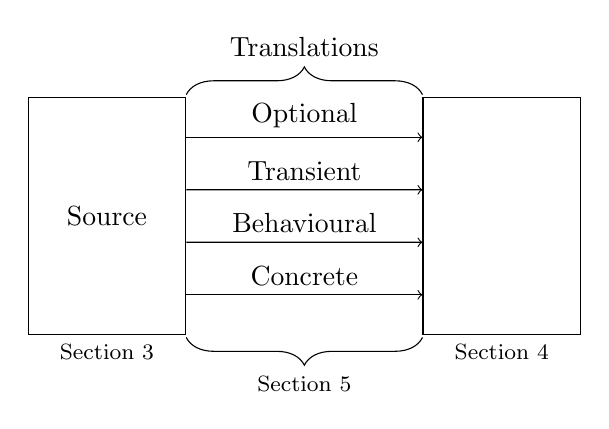
\begin{tikzpicture}[node distance=3cm]
\node[draw,minimum height=3cm,minimum width=2cm] at (0,0) (S) {Source};
\node[draw,minimum height=3cm,minimum width=2cm,right=of S] (K) {\kafka};
%\node[draw,right=of K] (C) {CIL};
\draw [->] ([yshift=1cm]S.east) -- node[midway,above] {Optional} ([yshift=1cm]K.west);
\draw [->] ([yshift=0.33334cm]S.east) -- node[midway,above] {Transient} ([yshift=0.3334cm]K.west);
\draw [->] ([yshift=-0.33334cm]S.east) -- node[midway,above] {Behavioural} ([yshift=-0.3334cm]K.west);
\draw [->] ([yshift=-1cm]S.east) -- node[midway,above] {Concrete} ([yshift=-1cm]K.west);

%\draw [->] (K) -- (C);

\draw [decorate,decoration={brace,amplitude=10pt,raise=1pt},yshift=0pt] (S.north east) -- (K.north west) 
  node [above,midway,yshift=0.4cm] {Translations};

\node[label,below=0cm of S] {\footnotesize Section 3};
\node[label,below=0cm of K] {\footnotesize Section 4};

\draw [decorate,decoration={brace,amplitude=10pt,mirror,raise=1pt},yshift=0pt] (S.south east) -- (K.south west) 
  node [below,midway,yshift=-0.4cm] {\footnotesize Section 5};
\end{tikzpicture}
\end{center}

We propose to compare approaches to gradual typing for objects by translating
a gradually typed source calculi to a traditionally sound target language, called
\kafka. \kafka is a statically typed class-based object calculus
with explicit mutable state. The key features of \kafka are casts:
\emph{structural casts} check if the object is a subtype of some type \t,
while \emph{behavioral casts} create wrappers, enforcing that an object
behaves as if it was of some type \t. By translating to this minimal
object-oriented calculus, we illustrate the source soundness guarantees 
provided by each semantics. Our approach is illustrated above.

This paper makes the following contributions:
\begin{itemize}  
  \item The design of \kafka, a common calculus for gradual type systems for
    objets.
\item Translations from a common source to \kafka implementing each gradual
  approach.
\item A litmus test comprised of three programs, able to tell apart the
  gradual type systems.
\item A mechanized proof of soundness of \kafka's type system, including
  class generation.
\item A proof-of-concept implementation of \kafka on the .Net Common
  Language Runtime.
\end{itemize}

\noindent Our work does not address the question of performance of the
translations. While there are intrinsic performance costs to the various
approaches, these costs could be mitigated by compiler optimizations.  A
significant difference with previous work is that \kafka is statically typed
-- other systems translate down to untyped calculi.  By translating to a
statically typed core, we can clearly see where wrapper-induced dynamic
errors can occur. Another design choice is the use of structural subtyping
in \kafka. This is motivated by our desire to represent behavioral and
transient approaches that require structural subtyping.  There would be no
major difficulty switching \kafka to a nominal subtype system or providing a
nominal subtype cast.

Our implementation and proofs are available from:
{\small \url{github.com/new_url}.}

\section{Background}

\epigraph{\vspace{-5mm}\small\it ``If you know the enemy and know yourself...''}

\vspace{-10mm}
\noindent The intellectual lineage of gradual typing can be traced back to
attempts to add types to Smalltalk and LISP. On the Smalltalk side, work on
the Strongtalk optional type system~\cite{Bracha93} led to Bracha's notion
of pluggable types~\cite{pluggabletypes}. For him, types exist solely to
catch errors at compile-time, never affecting the runtime behavior of
programs. The rationale is that types are an add-on that, when turned off,
do not affect program semantics.  In the term of Richards~\emph{et
  al.}~\cite{ecoop15}, an optional type system is \emph{trace preserving};
that is to say, if a term \e reduce to \a, then adding type annotations to
\e does not prevent \e from reducing to \a.  This property is valuable to
developers as it ensures that type annotations will not introduce errors.
Optional type systems in wide use include Hack~\cite{hack13},
TypeScript~\cite{BAT14} and Dart~\cite{dart13}.

Fellesien and his students have contributed substantially to functional
gradual typing. The Typed Scheme~\cite{tf-popl08} design that later became
Typed Racket is influenced by their earlier work on higher-order
contracts~\cite{ff-icfp02}. Typed Racket was envisioned as a vehicle for
teaching programming. Thus, being able to explain the source of errors was
an important design consideration. Another consideration was to prevent
surprises for beginning users, thus the value held in a variable annotated
with type \t should always behave as if it was of that type, this even when
transfered to a variable of another type. To aid debugging, any departure
from the expected behavior of an object, as defined by its behavioral type,
is reported at the first discrepancy.  Whenever a value crosses a boundary
between typed and untyped code, it is wrapped in a contract that monitors
its behavior. This ensures that mutable values remain consistent with their
declared type and functions respect their declared interface. When a value
misbehaves, blame can be assigned to a boundary. The granularity of typing
is the module, thus a module is either entirely typed or entirely untyped.

Siek and Taha coined the term gradual typing in~\cite{SiekTaha06} as ``any
type system that allows programmers to control the degree of static checking
for a program by choosing to annotate function parameters with types, or
not.'' Their contribution was a formalization of the idea in a lambda
calculus equipped with references. They defined the type consistency
relation $\t \sim \tp$ which states that types that agree on non-\any
positions are compatible.  In~\cite{SiekTaha07} the authors extended their
result to a stateless object calculus and combined consistency with
structural subtyping, but extending this approach to mutable objects proved
challenging. Reticulated Python~\cite{siek14} is a compromise between
soundness and efficiency.  The language has three modes: the \emph{guarded}
mode behaves as Typed Racket with contracts applied to values.  The
\emph{transient} mode performs shallow checks on reads and method returns,
only validating if the value obtained has matching method types.  The
\emph{monotonic} mode is fundamentally different from any of the other
previous approaches. Under the monotonic semantics, a cast updates the type
of an object in place by replacing some of the occurrences of \any with more
specific types, which can then propagate recursively through the heap until
a fixed point is reached.

Other noteworthy systems include Gradualtalk~\cite{GS13}, C\#
4.0~\cite{Bierman10}, Thorn~\cite{oopsla09}, Nom~\cite{Muehlboeck2017} and
Strong\-Script~\cite{ecoop15}. Gradualtalk is a variant of Smalltalk with
Felleisen-style contracts and mostly nominal type equivalence (structural
equivalence can be specified on demand, but it is, in practice, rarely
used). C\# 4.0 adds the type {\sf dynamic} to C\# and dynamically resolved
method invocation. Thus C\# has a dynamic sublanguage that allows developers
to write unchecked code, working alongside a strongly typed sublanguage in
which values are guaranteed to be of their declared type.  The
implementation replaces \any by the type {\tt object} and adds casts where
needed.  Thorn and StrongScript extend the C\# approach with the addition of
optional types (called {\em like types} in Thorn).  Thorn is implemented by
translation to the JVM. StrongScript translate to an extended version of
V8. The presence of concrete types means that the compiler can optimize code
(unbox data and in-line methods) and programmers are guaranteed that type
errors will not occur within concretely typed code. Nom is similar to Thorn
in that it is nominal and follows the concrete approach.

\newcommand{\rot}[1]{\rotatebox{80}{#1}\hspace{-10px}}
\newcommand{\X}{\EM{\bullet}}
\newcommand{\XX}{\EM{\bullet^{2}}}
\newcommand{\XY}{\EM{\bullet^{1}}}

\begin{figure}[!t]
  \center
  {\footnotesize
\begin{tabular}{r|lllllllllllllr}
 & & \rot{Nominal}
  & \rot{Optional}
  & \rot{Concrete}
  & \rot{Behavioral}
  & \rot{Class based}
  & \rot{First-class Class}
  & \rot{Soundness claim}
  & \rot{Unboxed prim.}
  & \rot{Subtype cast}
  & \rot{Shallow cast}
  & \rot{Generative cast}
  & \rot{Blame}
  & \rot{Pathologies}
  \\
Dart         &&\X &\X &   &   &\X &   &    &    &\X &   &   &   &  - 
\\\hline
Hack         &&\X &\X &   &   &\X &   &    &    &\X &   &   &   &  -  
\\\hline
TypeScript   &&   &\X &   &   &\X &   &    &    &   &   &   &   &  -  
\\\hline
C\#          &&\X &   &\X &   &\X &   &\XX & \X &\X &   &   &   &  -  
\\\hline
Thorn        &&\X &\X &\X &   &\X &   &\XX & \X &\X &   &   &   & 0.8x
\\\hline
StrongScript &&\X &\X &\X &\X &\X &   &\XX &    &\X &   &\X &   & 1.1x   
\\\hline
Nom 		 &&\X &   &\X &   &\X &   &\XX & \X &\X &   &   &   & 1.1x
\\\hline
Gradualtalk  &&\XY&   &   &\X &\X &   & \X &    &   &   &\X &\X &  5x
\\\hline
Typed Racket &&   &   &   &\X &\X &\X &\X  &    &   &\X &\X &\X & 121x 
\\\hline
Reticulated Python    \\
\it Transient&&   &\X &   &   & \X &  & \X &    &   &\X &   &\X & 10x \\
\it Monotonic&&   &   &   &\X & \X &  & \X &    &   &   &\X &\X &  27x\\
\it Guarded  &&   &   &   &\X & \X &  & \X &    &   &   &\X &\X &  21x\\
\end{tabular}}
  \caption{Gradual type systems. (1) Opt.~structural constraints. (2)
    Typed expressions are sound.}\label{over}
\end{figure}

\figref{over} reviews implemented gradual type systems for objects.  All
languages here are class-based, except TypeScript which has both classes and
plain JavaScript objects. That choice does not appear to be crucial, classes
are obvious source of type declarations.  Most languages build subtyping on
explicit subtype declarations -- nominal subtyping -- rather than on
structural similarities.  TypeScript uses structural subtyping, but does not
implement a runtime check for it.  Anecdotal evidence suggests that
structural subtyping is rarely needed in TypeScript~\cite{ecoop15},
Strong\-Script switches it to nominal for improved performance. While
nominal subtyping leads to more efficient type casts, Reticulated's
consistency relation is fundamentally structural; it would be nonsensical to
use it in a nominal system. Consistency relates classes that differ in the
number of occurrences of \any in their type signature and not whether they
are declared to extend one another.  For Racket, the heavy use of
first-class classes and class generation naturally leads to structural
subtyping as many of the classes being manipulated have no names and arise
during computation.

The optional approach is the default for Dart, Hack and TypeScript.
Transient Reticulated allows any value to flow in a field regardless of type
annotations, leading to its ``open world'' soundness
guarantee~\cite{siek14}.  In Thorn, Nom and C\#, primitives are concretely
typed; they can be unboxed without tagging.  The choice of casts follows
from other design decisions. The concrete approach naturally tend to use
subtype tests to establish the type of values. For nominal systems, there
are highly optimized algorithms. Shallow casts are casts that only check the
presence of methods, but not their signature. These are used by Racket and
Python to ensure some basic form of type conformance.  Behavioral casts are
used when information such as a type or a blame label must be associated
with a reference or an object.

Blame assignment is a topic of investigation in its own right. Anecdotal
evidence suggests that the context provided by blame helps developers
pinpoint the provenance of errors. A fitting analogy are the stack traces
printed by Java when a program terminates abruptly. Developers working in,
e.g, C++ must run their program in a debugger to obtain the same
information. Stack traces have little runtime cost because they piggyback on
precise exceptions. Recording blame has a cost, but no data exists on its
performance impact. We do not consider blame further in this paper.

The last column of \figref{over} lists self-reported performance
pathologies.  These numbers are not comparable as they refer to different
programs and different configurations of type annotations. They are not
worst case scenarios either; most languages lack a sufficient corpus of code
to conduct a thorough evaluation.  Nevertheless, one can observe that for
optional types no overhead is expected, as the type annotations are erased
during compilation. Concrete types insert efficient casts, and lead to code
that can be optimized.  The performance of the transient semantics for
Reticulated Python is a worst case scenario for concrete types -- i.e. there
is a cast at almost every call. Finally, languages with behavioral casts
tend to suffer prohibitive slow downs in pathological cases. Compiler
optimizations for reducing these overheads are an active research topic.
Languages such as C\#, Nom, Thorn, and Strong\-Script are designed to
exhibit minimal slowdowns. Typically the performance of fully typed code is
better than untyped code, and mixed code tend to performed well thanks to
relatively inexpensive nominal subtype tests.


%%%%%%%%%%%%%%%%%%%%%%%%%%%%%%%%%%%%%%%%%%%%%%%%%%%%%%%%%%%%%%%%%%%%%%%%%%%

\section{A Family of Gradually Typed Languages and their Litmus Test}\label{litmustest}

\epigraph{\vspace{-5mm}\small\it ``There is no perfection only life''} 

\vspace{-10mm}
\noindent
A consequence of the variety of approaches to gradual typing is there is no
single, common, notion of what constitutes an erroneous program. The choice
of enforcement strategy is reflected in the semantics of the language,
which, in turn, implies that developers have to understand the details of
the enforcement strategy if they want to avoid run-time errors.  This also
means that it is possible to differentiate between approaches by simply
observing the run-time errors that each type system produces.  We propose a
litmus test consisting of three programs whose execution depends on which
gradual type system is in use. Each of these program runs without error when
executed with a purely dynamic semantics, and each program is statically
well-typed. We start by presenting a common surface language in which we can
express our programs, and then explain why the various approaches to gradual
typing yield different run-time errors.

\subsection{A Common Surface Language}

\begin{figure}[!tb]\hrulefill

\small
\vspace{5mm}

{\bf Syntax:}\\[3mm]

\begin{tabular}{ll}
\begin{minipage}{6cm}\begin{tabular}{@{}l@{~}l@{}l@{}l@{}l@{}l@{}l@{}l}
\k~::=~ \Class \C {\fd[1]..}{\md[1]..} \qquad
\md~::=~\Mdef\m\x\t\t\e\qquad
\fd~::=~ \Fdef\f\t\qquad
\t~::=~ \any \B \C\\[3mm]
\e~::=~\x\B\this\B\FRead\f\B\FWrite\f\e\B\Call\e\m\e\B\New\C{\e[1]..}
\end{tabular}\end{minipage} 
\end{tabular}

\vspace{5mm}


{\bf Typing expressions:}\\[-6mm]

\begin{mathpar}
\Rule{STG-VAR}{~\\\\ 
  \HasType \Env\x\t
}{
  \EnvTypeS \Env\K\x\t
}

\Rule{STG-GET}{
  \HasType \Env\this\C \\\\  \Fdef\f\t \in \App\K\C
}{
  \EnvTypeS \Env\K{\FRead\f}\t
}    

\Rule{STG-SET}{
  \HasType \Env\this\C \quad \Fdef\f\t \in \App\K\C \\\\
  \EnvTypeS \Env\K\e\tp \quad  \ConvertE\K{s}\tp\t
}{
  \EnvTypeS \Env\K{\FWrite\f\e}\t
}    

\Rule[width=15em]{STG-CALL}{
  \EnvTypeS \Env\K\e\any \\\\ \EnvTypeS \Env\K\ep\t 
}{
  \EnvTypeS \Env\K{\Call\e\m\ep}{\any}
}    

\Rule[width=15em]{STG-CALL}{
  \EnvTypeS \Env\K\e\C \quad \EnvTypeS \Env\K\ep\t \\\\
  \Mtype \m{\t[1]}{\t[2]}\in \App\K\C  \quad
  \ConvertE\K{s}\t{\t[1]}
}{
  \EnvTypeS \Env\K{\Call\e\m\ep}{\t[2]}
}   

\Rule{STG-NEW}{
  \Ftype{\f[1]}{\t[1]}.. \in \App\K\C \\\\
  \EnvTypeS \Env\K{\e[1]}{\tp[1]}..\quad \ConvertE\K{s}{\tp[1]}{\t[1]}..
}{
  \EnvTypeS \Env\K{\New\C{\e[1]..}}\C
}
\end{mathpar}


{\bf Convertibility:}\\[-6mm]
  
\begin{mathpar}
\Rule{SUB}{ \SSub\emptyset\K\t\tp}{ \ConvertE\K{s}\t\tp }
    
\Rule{TOA}{~ }{ \ConvertE\K{s}\t\any}
    
\Rule{ANYC}{~}{ \ConvertE\K{s}\any\t }
\end{mathpar}


{\bf Subtyping:}\\[-6mm]

\begin{mathpar}
\Rule{SAss}{  }{  \StrSub \M\K \any\any }

\Rule{SAss}{ \C \Sub \D \in \M }{  \StrSub \M\K \C\D }

\Rule{SRec}{
\M'=\M~\C\Sub\D\\\\\md\in\App\K\D\implies\mdp\in\App\K\C~.~\StrSub{\M'}\K\md\mdp
}{
 \StrSub \M\K \C \D 
}

\Rule{SMet}{
  \StrSub \M\K{\tp[1]}{\t[1]} \qquad \StrSub \M\K{\t[2]}{\tp[2]}
}{
 \StrSub\M\K{\Mdef\m\x{\t[1]}{\t[2]}\e}{\Mdef\m\x{\tp[1]}{\tp[2]}\ep}
}
\end{mathpar}

\hrulefill
\caption{Surface language syntax and type system (extract).}\label{slts}
\end{figure}

We present a common surface language that can be used with different gradual
type systems. The surface language is a statically typed object calculus
without inheritance, method overloading or explicit type cast operations.
\figref{slts} gives its syntax and an extract of its static semantics. The
distinctive feature of the calculus is the presence of type \any\,-- the
dynamic type. A variable of type \any can hold any value, and an invocation
of a method with receiver of type \any is statically well-typed.

The presence of the dynamic type suffices to allow writing gradually typed
code. A program with no occurrence of \any is statically typed, in which
case, the usual soundness guarantee holds, namely programs will not get
stuck on method invocation. A program where all variables are annotated as
dynamic is fully dynamic and any invocation may get stuck.
Gradual typing comes into play when an expression of type \any occurs as an
argument to a method that expects some other type \C and conversely when an
argument of type \C is passed to a method that expects \any. The static type
system of the surface language allows such implicit coercions, but run-time
checks may be inserted to catch potential type mismatches. The following
sections formalize the semantics of the different gradual approaches in
terms of a translation into \kafka, our lower-level common calculus.  In
this section, we appeal to the reader's intuition.

Before presenting the litmus test, some details about the type system of the
surface language may prove helpful. The subtyping relation is structural
with the Amber rule~\cite{cardelli1985amber}, \StrSub\M\K\C\D holds if class
\C has (at least) all the methods of class \D and the arguments and return
types are related by subtyping in the usual contra- and co-variant way; the
class table \K holds definitions of all classes and \M is helper for
recursion. One noteworthy feature of subtyping is that the fields of objects
do not play a role in deciding if classes are subtypes. Following languages
like Smalltalk, fields are encapsulated and can only be accessed from their
defining object, syntactically field reads and write are limited to
\this.\f. The static type-checking rules are standard with two exceptions.
Method invocation, \EM{\e.\m(\ep)}, when the receiver is dynamic,
\EM{\e:\any}, allows the invocation of any method \m, with a dynamic
argument, \EM{\ep:\any}, and a dynamic return type, \EM{\e.\m(\ep):\any}.
Mixing static and dynamically typed terms is achieved by implicitly
converting typed and untyped terms. The convertibility relation, written
$\ConvertE\K s\t\tp$, states that type $\t$ is convertible to type $\tp$
assuming class table \K.  The relation is used both for up-casting and for
conversions of \any to non-\any types.  $\ConvertE\K s\t\tp$ holds when
$\t\Sub\tp$, this allows up-casts. The remaining two rules allow implicit
conversion to and from the dynamic type.  To avoid collapsing the type
hierarchy, convertibility is not transitive. Implicit conversion break
soundness, their use motivates the need for dynamic checks.  If some typed
term is passed into untyped code, it must be protected from
misuse. Likewise, if an untyped term is passed into typed code, then type
invariants must be checked.


\subsection{Litmus}

Using three different programs, we can differentiate between four gradual
type systems. The litmus test is shown in \figref{litmus} and its
constituent programs are written in our surface language.  Each of these
programs consists of a class table and an expression, whose evaluation in
the context of the class table determines if the litmus test succeeds or
fails.

The programs are designed to induce errors.  This is done via the
construction of an untyped value that violates the type guarantees of some
systems, but not others.  At heart, these programs can be summarized by the
typed/untyped boundaries that are crossed by an object. Let us use the
notation $\C ~\vert_{\,\t}$ to denote that an object of class \C passes
through a type boundary that expects it to be of type \t.  In program {\bf
  L1}, we have \[\A ~\vert_{\,\any} ~ \vert_{\,\I}\] an instance of class \A is
first implicitly converted to \any and then to \I. Classes \A and \I are
unrelated by subtyping. In program {\bf L2}, the same sequence is applied
\[\A~ \vert_{\,\any} ~ \vert_{\,\I}\] but this time \A and \I both have method
\m, but with incompatibly argument types. Lastly, in program {\bf L2}
we start by converting an object of class \C to \any and then to \E and
finally back to \any.
\[\C~ \vert_{\,\any}~\vert_{\,\E}~\vert_{\,\E}~\vert_{\,\any}\]
the resulting value is then used in a call to method \m with an instance of
\C as an argument. This call is correct as method \m in \C does take an
argument of the same type. If the object was an instance of \E, the call
would not be legal because \E's method \m expects a class \D as argument.

\begin{figure}[!h] 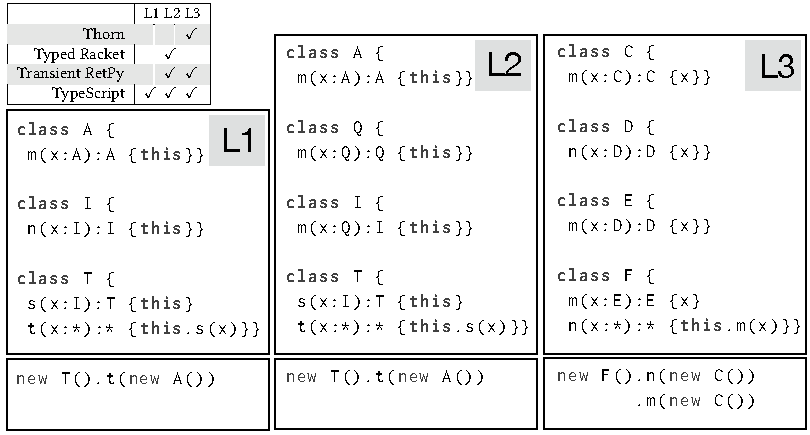
\includegraphics[width=.95\columnwidth]{../figures/litm}
  \caption{Gradual typing litmus test.}\label{litmus}
\end{figure}

\vspace{2mm}\noindent
{\bf Optional.~} An optional gradual type system simply erases all of the
type annotations at run-time; all three programs run to completion without
error.

\vspace{2mm}\noindent {\bf Concrete.~} The guarantee provided by the
concrete semantics is that all implicit conversion imply a run-time subtype
check.  This causes all three programs to experience failure. {\bf L1} and
{\bf L2} fail on a subtype test \StrSub{}\K\A\I.  {\bf L3} fails on the
subtype test \StrSub{}\K\C\E.

\vspace{2mm}\noindent {\bf Behavioral.~} The behavioral semantics does allow
conversion from \any to \C if the actual value is ``structurally''
compatible to \C and if, after that, the value ``behaves'' as if it was an
instance of \C.  This is checked by a run-time cast that looks at method
names and a wrapper that monitors further interactions.  {\bf L1} is rejected
because \A does not have the method \xt n expected by \I. {\bf L2}, however,
executes without error because \A has the method \m expected by \I (argument
types are not checked). {\bf L3} is fails, the instance of \C has been
applied a wrapper that checks it behave as if it was an instance of \E.
When the method \a is called with a \C object as argument, the wrapper will
observe that \E has a method \a but that method expects a \D and \C and \D
are not compatible.

\vspace{2mm}\noindent {\bf Transient.~} The transient semantics has a weaker
guarantee, It retains the structural checks at casts of the behavioral
semantics, but does not wrap values. Transient fails {\bf L1}, for the same
reason as the other two type systems, and passes {\bf L2}, for the same
reason as the behavioral semantics.  {\bf L3} succeeds because transient
forgets that the \C object was converted to \E.

\subsection{Discussion}

The litmus tests also capture the behavior of real languages. These tests
programs have been expressed in TypeScript (optional), StrongScript
(concrete), Typed Racket (behavioral) and Reticulated Python
(transient).\footnote{http://github.com/FIXME} Those implementations have
the same errors.

What the litmus tests show is that understanding the implementation of
gradually typed languages, the run-time enforcement machinery, is crucial
for developers to know, precisely, when their programs is ``correct''.  In
the case of the litmus, all errors are spurious, none of these programs is
incorrect. This points to the fact that in gradually typed language, bugs
can slip into the type specification and those bugs can cause run-time
errors. Thus, type annotations must be audited and tested just like code.

There are clear usability trade-offs between approaches. The optional
approach is the most permissive, developers need not worry about type
annotations introducing bugs as annotations have no impact on program
execution. On the other hand, any method invocation may go wrong. So the
guarantees provided by this approach are the weakest. The behavioral
approach was designed to be sound, this comes at the cost of not being able
to rule out run-time errors at any operation. The use of wrappers to monitor
the behavior of values has the consequence that any method invocation may
fail if the receiver is a wrapped object.  Concrete types have a much
simpler semantics, errors only occur at the boundary between untyped and
typed code. Method invocation on a typed receiver with typed arguments will
never get stuck. The concrete approach is more restrictive as the values
that cross a typed boundary must be related by subtyping to expected type.
Finally the transient approach occupies a middle ground with weaker
guarantees than behavioral and less restrictions than concrete.

Reticulated Python uses a \emph{consistency} relation instead of
subtyping~\cite{siek14}.  Consistency allows to treat accept more programs
as types that have fewer occurrences of \any are consistent with types that
have more \any. But consistency does not affect the run-time semantics of
the transient approach, so we omit it here. Consistency is not compatible
with the concrete approach. As for behavioral, the Type Racket incaranation
expects code to be either fully or fully untyped, in which case consistency
boils down to subtyping.

Thorn and StrongScript combine the concrete and optional approach as they
support three kinds of types, \any (dynamic), \C (concrete) and \xt{like} \C
(optional). The run-time semantics matches that of the concrete approach.

The choice of structural subtyping for the surface language is motivated by
the desire to support the transient approach. For the concrete approach a
nominal subtyping relation is more natural (and used in Nom, Thorn and
StrongScript).

The motivation for private fields is to simplify the system. With private
fields, errors are limited to method invocation. Fields accesses can be
trivially checked. Moreover, interposing on method invocation can easily be
achieved by wrappers, whereas interposiing on field access would require
modifying the code of clients. This would make the formal development more
cumbersome without adding much insights.


%%%%%%%%%%%%%%%%%%%%%%%%%%%%%%%%%%%%%%%%%%%%%%%%%%%%%%%%%%%%%%%%%%%%%%%%%%%
\section{KafKa: A Core Calculus}\label{kafkacore}

\epigraph{\it ``Aux chenilles du monde entier et aux papillons qu’elles
  renferment''}

\noindent Even without gradual typing, it is difficult to compare languages.
Small differences in syntax and supported features can make even the most
similar languages appear different. As a result, the nuances of gradual type
systems are often hidden amongst irrelevant details.  To enable direct
comparison, we propose to translate gradual typed languages down to a common
calculus, named \kafka, designed to highlight the distrinctions between
gradual type systems for objects.

One goal is to explicit the guarantees provided by the surface language.  To
this we designed a target language, \kafka, that is statically typed and
that two dedicated cast operations. It makes a syntactic distinction between
dynamic method invocation, written \KCall\e\m\ep\t\tp, and static
invocation, written \DynCall\e\m\ep. The static type system ensures that
static invocations will not go wrong, whereas any dynamic invocation may get
stuck. The two cast operations include a standard structural subtype cast,
written \SubCast\t\e, that ensure the object that expression \e evaluates to
is a subtype of \t, and a behavioral cast, written \BehCast\t\e, that
creates a wrapper around an object that monitors that it indeed behave as
according to type \t. The translations from the source language to \kafka
precisely describe the enforcement machinery required by each gradual
approach.

\kafka was also designed to align with the capabilities of compilation
target such as .NET or the JVM. It is a class-based, object-oriented,
statically typed language, that support dynamic code generation. This last
feature is somewhat unsual for formal calculi, but required to express
behavioral casts.


%%%%%%%%%%%%%%%%%%%%%%%%%%%%%%%%%%%%%%%%%%%%%%%%%%%%%%%%%%%%%%%%%%%%%%%%%%%%
\begin{figure}[!h]\small\noindent\hrulefill

\vspace{4mm}
{\bf Syntax:}
\vspace{2mm}

\begin{tabular}{@{}ll}\hspace{5mm}\begin{minipage}{7.2cm}\begin{tabular}{@{}l@{~}l@{}l@{}l@{}l@{}l@{}l@{}l}
\e\hspace{.1cm} ::=  \hspace{.2cm} 
 & \x       &\B \this       &\B \that  & \B   \\
 & \FRead\f &\B \FWrite\f\e &\B \New\C{\e[1]..} &\B\\
 & \KCall\e\m\e\t\t   &\B \DynCall\e\m\e &\B\\
 & \SubCast\t\e  &\B \BehCast\t\e & \B \\
 &  \a  &\B \FReadR\a\f &\B \FWriteR\a\f\e 
\end{tabular}\end{minipage}&
\begin{minipage}{2.4cm}\begin{tabular}{l@{~}l@{}l@{}l}
  \k &::= \Class \C {\fd[1]..}{\md[1]..} \\
 \md &::= ~ \Mdef\m\x\t\t\e \\ 
 \fd &::= ~ \Fdef\f\t \\ 
  \t &::= ~ \any  \B   \C  \\ 
\end{tabular}\end{minipage}\end{tabular}

\vspace{6mm}
{\bf Static semantics:}
\vspace{-2mm}

\begin{mathpar}
\Rule{W6}{
  \EnvType \Env\s\K\e\C \\
  \Mtype\m\t\tp \in \App\K\C  \\
  \EnvType \Env\s\K\ep\t
}{
  \EnvType \Env\s\K{\KCall\e\m\ep\t\tp}\tp
}    

\Rule{W7}{
  \EnvType \Env\s\K\e\any \\
  \EnvType \Env\s\K\ep\any
}{
  \EnvType \Env\s\K{\DynCall\e\m\ep}\any
}    

\\

\Rule{W9}{
  \EnvType \Env\s\K\e\tp
}{
  \EnvType \Env\s\K{\SubCast\t\e}\t
}

\Rule{WB}{
  \EnvType \Env\s\K\e\tp
}{
  \EnvType \Env\s\K{\BehCast\t\e}\t
}

\Rule{W9}{
  \s(\a) = \obj\C{\ap[1]..}
}{
  \EnvType \Env\s\K\a\C
}

\Rule{W10}{
 }{
   \EnvType \Env\s\K\a\any
}
\end{mathpar}


\vspace{4mm}
{\bf Execution contexts:}
\vspace{-2mm}

\[
\begin{tabular}{llllllllllllllllll}
\EE &::=& ~ \FWriteR\a\f\EE   &\B  
        \KCall\EE\m\e\t\t  &\B
        \KCall\a\m{\EE}\t\t &\B
        \DynCall\EE\m\e   &\B\\
&       & \DynCall\a\m\EE   &\B
       \SubCast\t\EE  &\B
      \BehCast\t\EE  &\B
       \New\C{\a[1]..\,\EE\,\e[1]..} &\B 
      \EM{\square}
\end{tabular}
\]

\vspace{4mm}
{\bf Dynamic semantics:}
\vspace{2mm}

\hspace{7mm}\begin{minipage}{\textwidth}

\begin{tabbing}
  \K\HS \New\C{\a[1]..} \HS\= \s~ \HS \=\Red\HS \= \K \HS\= \ap \HS\= \sp\HS \= \WHERE\HS\= \fresh\ap \HS\HS\HS\HS\HS\HS\HS\=  \sp = {\Map\s{\Bind\ap{\obj\C{\a[1]..}}}}
\\
\K\HS \FReadR\a{\f[i]} \> \s           \>\Red\>     \K \>$\a[i]$ \> \s  \> \WHERE \>\App\s\a=\obj\C{\a[1],\ldots\a[i],\a[n]\ldots}
\\
\K\HS {\FWriteR\a{\f[i]}\ap} \> \s     \>\Red\>     \K \> \ap \> \sp \>  \WHERE \>\App\s\a=\obj\C{\a[1],\ldots\a[i],\a[n]\ldots} \HS  
\\ \> \> \> \> \> \> \> \sp = \Map\s{\Bind\a{\obj\C{\a[1],\ldots\ap,\a[n]\ldots}}}
\\
\K\HS{\KCall\a\m\ap\t\tp} \> \s      \>\Red\>     \K \>  \ep \> \s \> \WHERE\> \ep = {[\a/\this~{\ap/\x}]\e} \HS \\ \> \> \> \> \> \> \> \Mdef\m\x{\t_{1}}{\t_{2}}\e\In \App\K\C  \\ \> \> \> \> \> \> \>  \App\s\a=\obj\C{\a[1]..} \> \StrSub {\emptyset}\K\t {\t_{1}} \\ 
\> \> \> \> \> \> \> \StrSub {\emptyset}\K{\t_{2}} \tp
\\
 \K\HS {\DynCall\a\m\ap}\> \s        \>\Red\>    \K \> \ep \> \s \>  \WHERE\> \ep = {[\a/\this~{\ap/\x}]\e}\HS \\ \> \> \> \> \> \> \> \Mdef\m\x\any\any\e \In \App\K\C \\ \> \> \> \> \> \> \> \App\s\a=\obj\C{\a[1]..} 
\\
 \K\HS {\SubCast \any\a} \> \s       \>\Red\>   \K \> \a \> \s
\\
 \K\HS {\SubCast \D\a} \> \s        \>\Red\>    \K \> \a \> \s \>  \WHERE\> \StrSub {\emptyset}\K\C \D \>\App\s\a=\obj\C{\a[1]..} 
\\
 \K\HS {\BehCast \t\a} \> \s         \>\Red\>   \Kp \> \ap \> \sp \> \WHERE\> \behcast \a\t\s\K \Kp\ap\sp    
\\
\K \HS \EM{\EE[\e]} \> \s            \>\Red\>   \Kp \> \EM{\EE[\ep]} \> \sp \> \WHERE \> \K~\e~\s \Red~\Kp~\ep~\sp
\end{tabbing}
\end{minipage}

\medskip
\hrulefill
\caption{\kafka dynamic semantics and static semantics
  (extract).}\label{fig:kafka}
\end{figure}


\subsection{Syntax and Semantics}

\kafka has two key requirements. First, it needs to be able to express the
dynamic semantics implied by each gradual type system. Second, it should
have a type system that can capture some cases when code can be statically
shown to be error free.  Syntax and semantics of the calculus appear in
\figref{fig:kafka}. They are loosely inspired by  Featherweight Java~\cite{}.
At the top level, classes are notated as \Class\C{\fd[1]..}{\md[1]..},
methods, ranged over by \md, are denoted as \Mdef\m\x\t\t\e, and fields
\Fdef\f\t. Expressions consist of

\vspace{-2mm}

\begin{itemize}
\item variable references, \x;
\item self-reference \this, and wrapped reference, \that;
\item field access, \FRead\f, and writes, \FWrite\f\e;
\item object creation, \New\C{\e[1]..};
\item static and dynamicd method invocations;
\item subtype and behavioral casts;
\item references, assignment, and dereference forms for runtime use.
\end{itemize}

\noindent
Evaluation is mostly standard with an evaluation context consisting of a
class table \K, an expression being evaluated \e, and a heap \s, mapping
from addresses \a to objects, denoted $\C\{\a\ldots\}$. Due to the need for
dynamic code generation, the class table is part of the state.  The
treatment for majority of these constructs are orthogonal to the issues
related to supporting gradual typing, therefore their semantics are typical
for calculi of this style.  Calls and casts, however, are atypical.

\kafka's static semantics hold few surprises. The key typing rules appear in
\figref{fig:kafka}. The subtyping relation is inherited from the surface
language.  The program typing relation (not shown here), \WFp\e\K, indicates
that expression \e is well-formed with respect to class table \K, and the
expression typing judgment $\EnvType \Env\s\K\e\t$, indicaties that against
\Env, with heap \s, and class table \K, \e has type \t.  Unlike the surface
language, \kafka does not rely on a convertibility relation to from \any to
\C and back.  Instead, explicit casts are required. The subtype cast
\SubCast\t\e and behavioral cast \BehCast\t\e both allow to retype an
expression of some type \tp as type \t without any static checks. The type
rule for dynamic method invocation \DynCall\e\m\ep allows the invocation of
any method \m on a receiver and argument of type \any, and has a return type
of \any.

\subsubsection{Method Invocation}

\kafka has two invocation forms, the dynamic \DynCall\e\m\ep and the static
\KCall\e\m\ep\t\tp, both denoting a method call to method \m with argument
\ep.  There several design issues worth discussing.  First, as our calculus
is the target of translation, we require some explicit prepartion for
objects to be used in a dynamic context.  A dynamic call is only sucesfull
if the receiver has a method of the expected name which take an argument of
type \any and returns a value of type \any. Thus, even the dynamic
invocation has to be well-typed. Secondly, it is possible for a static
invocation to call a method of type \any.  Consider the following definition

\newcommand{\Int}{\xt{Int}}

\begin{tabbing}
\small\hspace{2cm}\class \C \=\{\\
 \>\HS\HS\Mdef\m\x\Int\Int{\HS\x+2\HS}\\
 \>\HS\HS\=\m(\x:~\any)~:~\any\{~\SubCast\any{\KCall\this\m{\SubCast\Int\x}\Int\Int}~\}\\
     \> \}
\end{tabbing}

\noindent
and assume that that the class table \K holds a definition for \xt{Int},
furthermore we take liberties with syntax around addition and integers for
illustration.

Class \C demonstrates several features of \kafka. It's class well-formdness
rules (not shown here) allow a limited form of method overloading. A class
may have at most two occurences of any menthod \m. One, which we call
``untyped'', with \any as argument and return type. And one, which call
``typed'', with either argument and/or return type different from \any.
The static type system enforces a single means of invoking
a typed method \m:

\vspace{-6mm}\[\KCall{\New\C{}}\m{2}\Int\Int\] \vspace{-5mm}

\noindent
Here the reciever is obviously of type \C and the argument is \Int, thus the
call is statically well-typed. The expression is thus guaranteed to evaluate
the body of \m.  For an untyped method, there are two invocation modes:

\vspace{-6mm}\[\DynCall{\New\C{}}\m{2}\]\vspace{-5mm}

\noindent in a dynamic invocation, the method may be missing, and thus
evaluation may get stuck. On the other hand, one could use  static
method invocation form such as

\vspace{-6mm}\[\KCall{\New\C{}}\m{2}\any\any\]\vspace{-5mm}

\noindent then the receiver is checked to have a method \m from \any to
\any, and the invocation is guaranteed to succeed. All of the nuances will
come in handy when translating the surface language to \kafka.

\subsubsection{Run-time Casts}

\kafka has two cast operations: the subtype cast $\SubCast\t\e$ and the
behavioral cast $\BehCast\t\e$, both indicating the desire that the result
of evaluating \e has type \t.  Where the two casts differ is what is meant
by ``has type \t''.  The subtype casts checks that the result of evaluating
\e, is an object whose class is a subtype of \t. If \SubCast\t\e succeeds,
then the value it returns is of type $\t$ or, if the \EM{\t=\any} then the
subtype cast is trivially succesful. This cast is possible because every
value in the heap is an object made up of a class \C and a list of field
values. The behavioral cast is more complex, we will describe it in the
remainder of this section.

The behavioral cast wraps the result of evaluating \e in a newly created
object which enforces the invariant that it \emph{behaves as} a value of
type \t.  The semantics of this cast are implemented by function
\behcastE\a\t\s\K \Kp\ap\sp shown in \figref{behavetext}.  There are two
cases to consider, either the type to enforce is a class \Cp, or it is \any.

\begin{figure}[!h]\hrulefill\small

\vspace{4mm}
{\bf Behavioral cast:}
\vspace{4mm}
\behcastE\a\t\s\K \Kp\ap\sp\\[2mm]
\begin{tabular}{ll|ll}
\a & Reference to wrap & \ap & Wrapped reference \\
\t & Type to enforce & \Kp & Class table with wrapper\\ 
\s & Original heap & \sp & New heap \\
\K & Original class table &
\end{tabular}

\vspace{4mm}

\begin{equation*}
\behcastE\a\Cp\s\K \Kp\ap\sp \HS\WHERE\HS \begin{cases}
 \HS\App\s\a = \obj\C{\a[1]..} \HS\HS    \fresh{\D,\ap} \HS\HS
  \sp = \Map \s{\Bind\ap{\obj\D{\a}}} \\\HS
  \md[1].. \In\App\K\C \HS\HS \names{\mdp[1]..} \subseteq \names{\md[1]..} \\\HS
  \mdp[1].. \In \App\K\Cp \HS\HS \cload{\md[1]..} \HS \cload{\mdp[1]..} \\\HS
  \Kp = \K ~\wrap\C{\md[1]..}{\mdp[1]..}\D 
  \end{cases}
\end{equation*}

~\\[-8mm]

\begin{equation*}
  \behcastE\a\any\s\K \Kp\ap\sp  \HS\HS\WHERE\HS\HS\begin{cases}\HS
  \App\s\a = \obj\C{\a[1]..} \HS\HS \md[1].. \In \App\K\C \HS\HS
  \fresh{\D,\ap} \\\HS \cload{\md[1]..} \HS\HS
  \Kp = \K ~ \wrapAny\C{\md[1]..}\D \\\HS
  \sp = \Map \s{\Bind\ap{\obj\D{\a}}} 
\end{cases}\end{equation*}

\vspace{4mm}

\hspace{8mm}\begin{minipage}{12cm}\begin{tabbing}\small
  \wrap\C{\md[1]..}{\mdp[1]..}\D = \src{\Class\D{\Fdef\that\C}{\mdpp[1]..}}\\
  \HS\HS\WHERE\HS\= \Mdef\m\x{\t[1]}{\t[2]}\e\In\md[1].. \\
                 \> \mdpp[1] =\= \src{\Mdef\m\x{\tp[1]}{\tp[2]}{~\BehCast{\tp[2]}{\KCall{\FRead\that}\m{\bscast{\tp[1]}\x}{\t[1]}{\t[2]}}}} .. \\
\> \> \HS\HS \= \textbf{if} \HS \Mdef\m\x{\tp[1]}{\tp[2]}\ep\In\mdp[1].. \\
\\[-3mm]
\> \>  \src{\Mdef\m\x{\t[1]}{\t[2]}{~\KCall{\FRead\that}\m{\x}{\t[1]}{\t[2]}}} .. \\ \> \> \HS\HS \textbf{otherwise}
\\[2mm]
  \wrapAny{\C}{\md[1]..}{\D} = \src{\Class \D{ \Fdef\that\C}{ \mdp[1]..}}\\
\HS\HS\WHERE\HS\=\mdp[1] = \src{ \Mdef\m\x{\any}{\any}{~\BehCast\any{ \KCall{\FRead\that} \m {\bscast{\t}\x}{\t}{\tp}} } }   ..
    \HS\HS\HS\HS \\ \> \> \HS\HS \= \textbf{if} \HS \Mdef\m\x{\t}{\tp}\e\In\md[1].. \\
\end{tabbing}\end{minipage}

\vspace{-2mm}

\hrulefill
\caption{Behavioral casts semantics.}\label{behavetext}
\end{figure}

\newcommand{\W}{\xt{W}\xspace}

If the target type is \Cp, then \behcastS\a\Cp\s\K will return an updated
class table \Kp, a reference to the wapped object \ap, and an updated heap
\sp. The only property immediately checked is that the object referenced by
\a has all of the method names declared by \Cp. If this is not the case, it
is impossible for the obejct to implement the desired interface so an early
failure is acceptable. The function will generate a wrapper, that is, it
generates code for a new class for the wrapper object, instantiates it, and
returns a wrapper \ap that points to \a. The metafunction \W does the heavy
lifting of class creation. The metafunction is used as follows,
\EM{\W(\C,\md_1..,\mdp_1.., \D)} takes a class \C, a fresh name \D, and two
method lists $\md_1..$ and $\mdp_1$, respectively the method of \C and the
methods of the type to enforce.  The generated class will have adapter
methods for each method \m occurring in both $\md_1..$ and $\mdp_1..$.  The
adapter will introduce behavioral casts for argument and return values.  For
method that do not need to be adapted (methods only in $\md_1..$) as simple
pass-through method is generated that calls the target.  The translation
uses distinguished variable \that to refer the wrapped object.

If the target type is \any, the wrapper class is simpler. It need to check
that the argument type matches the type expected by the wrapped object. This
is done by a behavioral cast. Return values are behaviorally cast to \any.



For example, consider the following:

\begin{tabbing}
\hspace{1cm}\K\HS
\Call{(\BehCast\C{(\BehCast\D{\New\C{}})})}{\xt{b}}{2} \HS\HS\HS\WHERE\HS
  \K\HS =\HS \= \class\= \C \{\\
       \> \HS \Mdef{\xt{a}}\x\any\any{\HS\x\HS}\\
       \> \HS \Mdef{\xt{b}}\x\any\any{\HS\x\HS}\\
       \> \}  \\
       \>\class \D \{\\
       \> \HS \Mdef{\xt{a}}\x{\xt{Int}}{\xt{Int}}{\HS\x\HS}\\
       \> \}
\end{tabbing}

In this example, we start with an instance of \C, cast it to \D, which only
has one of \C's two methods, then cast it back. One interpretation would be
to generate a wrapper at the first cast that does not include \xt{b}, as it
is not required to implement \D, but then this would cause the second cast
to fail.  As a result, if there is some \m that is not specified in \mdp[1],
the typed W implementation will simply pass calls to it through the
wrapper. This is still safe, as the wrapper's pass-through method for \m has
the same types as the original \m, and allows the above example to succeed.


\subsection{Type soundness}

Type soundness is a key property of the \kafka type system, as if the
soundness of gradual type systems is to be represented in terms of it, then
it follows that \kafka must itself be type safe.  The \kafka type soundness
theorem is stated as follows:

\begin{theorem}[\kafka type soundness]

\noindent For every well-formed-state $\WFq{\K~\e~\s}$ and well-typed expression
$\EnvType\emptyset\s\K\e\t$, one of the following holds:

\begin{itemize}
\item There exists some reference $\a$ such that $\e = \a$.
\item $\K~\e~\s \Red \Kp~\ep~\sp$, where $\WFq{\Kp~\ep~\sp}$, $\EnvType\emptyset\sp\Kp\ep\t$, $\sp$ has all of the values of $\s$, and $\Kp$ has all of the classes of \K.
\item $\e=E[\DynCall\a\m\ap]$ and $\a$ refers to an object without a method \m.
\item $\e=E[\SubCast\C\a]$, and $\a$ refers to an object whose class is not a subtype of $\C$.
\item $\e=E[\BehCast\C\a]$, and $\C$ contains a method that \a does not.
\end{itemize}
\end{theorem}

As such, a valid \kafka program can only get stuck at a dynamic invocation, a
subtype cast, or a behavioral cast, and only there when justified, which in turn
enables us to reason about the semantics of the gradual type systems by reasoning
about the type of their \kafka translation.

The proof is mostly straightforward, with one unusual case, centered around
the \xt{bcast} metafunction. When the expression $\BehCast\C\a$ is
encountered, the \xt{bcast} metafunction is used to generate a wrapper class,
which is then instantiated, producing a new class table, return value, and
heap. We must then show that the new class table is well formed, that the new
heap is also well formed, and that the new wrapper is a subtype of the given
type $\C$. 

Proving these properties is relatively straightforward. Class table well-
formedness follows by construction of the wrapper class and by well-formedness
of the old class table. Heap well-formedness follows by well-formedness of the
class table, construction of the new heap, and well-formedness of the old heap.
Lastly, proving that the type of the wrapper is a subtype of the required type
proceeds by structural induction over the required type.

The proof of soundness for our type system has been formalized in Coq, which
can be found in the supplementary material for this paper. Our proof has two
key axioms: recursive structural subtyping is transitive and correct. We did
not prove these assumptions (which have been shown in prior
work~\cite{JonesStructural}) as they lie outside the scope of our project.

Type soundness is only one means of validating a language design and type
system, however, as while it demonstrates that reasoning about types only need
be done in \kafka, it does not demonstrate the practical applicability of 
lessons learned from translations to \kafka, which needs a different approach.


\subsection{Discussion}



Traditionally, dynamic invocations are represented in gradual type translation
targets through the combination of a cast and a normal typed invocation. For
example, to call an untyped method \m with value \e, Vitousek, Swords, and
Siek 2017~\cite{Vitousek2017} would represent it as $(\SubCast{\any
\rightarrow\any}{\m})(\e)$, casting the receiver to an arrow type then 
performing a (sound) invocation. 

In order to generate such a cast, we need to produce a type that guarantees
the existence of the corresponding method. If we attempt to translate the
above example into \kafka, without knowing anything about the context, we run
into a substantial problem: types can only be declared in the class table.
Instead, if we are trying to invoke a method \m on receiver \a with argument
\e, we have to assume the existence of a class similar to $\Class{\xt
M}{}{\Mdef\m\x\any\any\x}$ in the class table, from which we can then write
$\KCall{\SubCast{\xt M}\a}\m\any\any\e$. However, this class needs to be
generated by the translation, adding substantial complexity.

Instead, we simply treat the untyped invocation form separately, specifying
that it will always call an untyped method and that it may fail, as discussed
later in our discussion of the \kafka soundness proof.


Our use of explicitly typed invocations is a result of the desire for \kafka
to be the target of multiple gradual type systems and the corresponding
requirement of generality, and arises from the need to protect typed method
from untyped callers in the concrete semantics.

Consider the following example:


\begin{tabbing}
\hspace{1cm}\K\HS\=
\Call{\New\C{}}{\m}{2} \HS\HS\HS\HS\HS\HS\HS\HS\HS\HS\WHERE
  \K\HS =\HS \= \class\= \C \{\\
\> \Call{(\SubCast\any{\New\C{}})}{\m}{\xt{"hello"}}       \> \HS \Mdef{\xt{m}}\x {\xt{Int}}{\xt{Int}}{\HS \x + 2 \HS}\\
   \>    \> \}
\end{tabbing}

The intuition for the first invocation of \m is clear - the method \m in
class \C is called.  However, the second invocation is less obvious. If we
interpret the untyped invocation as calling \m directly, then it is clear
that the types are not sound, and some mechanism is needed to intercede upon
this untyped invocation.  This could be treated as a special case of untyped
invocation, an approach taken in many gradual type systems dedicated to one
language~\cite{popl10,ecoop15,Muehlboeck2017}.

This approach is untenable for multiple gradual type systems cohabiting in a
single language. Fixing the untyped invocation semantics as part of basic
semantics precludes  the use of different enforcement mechanisms, protecting
typed from untyped code. Moreover, it hides an important set of type tests, 
obscuring a potential source of type errors.

\begin{itemize}
  \item Globally consistent renaming, introducing a new untyped method for
    each typed method, and renaming every untyped method consistently. Under
    this scheme, every dynamic invocation can be translated to invoke
    functions under their untyped names. Using this approach, and denoting
    the untyped method name corresponding to \m as \mp, the example would
    become


\begin{tabbing}
\hspace{1cm}\K\HS\=
\Call{\New\C{}}{\m}{2} \HS\HS\HS\HS\HS\HS\HS\HS\HS\WHERE\HS
  \K\HS =\HS \= \class\= \C \{\\
\> \Call{(\SubCast\any{\New\C{}})}{\mp}{\xt{"hello"}}       \> \HS \Mdef{\m}\x {\xt{Int}}{\xt{Int}}{\HS \x + 2 \HS}\\
\>\>\HS \=\mp(\x:~\any)~:~\any \{ \\
\>\>\>\HS\HS\HS\SubCast\any{\Call\this\m{\SubCast{\xt{Int}}}} \HS\}\\
   \>    \> \}
\end{tabbing}

This is fully unambiguous, but the requirement for this globally-unique,
always-free name translation adds substantial complexity to the formalism.
\item Type-based overloading of methods, where the typed invocation form can
  choose between methods of the same name but different type signatures,
  while the untyped invocation always calls the untyped method. Using this
  approach, the code becomes

\begin{tabbing}
\hspace{1cm}\K\HS\=
\KCall{\New\C{}}{\m}{2}{\xt{Int}}{\xt{Int}} \HS\HS\HS\HS\HS\WHERE~
  \K ~=~ \= \class\= \C \{\\
\> \KCall{(\SubCast\any{\New\C{}})}{\m}{\xt{"hello"}}\any\any \> \HS \Mdef{\m}\x {\xt{Int}}{\xt{Int}}{\HS \x + 2 \HS}\\
\>\>\HS \=\mp(\x:~\any)~:~\any \{ \\
\>\>\>\HS\HS\HS\SubCast\any{\KCall\this\m{\SubCast{\xt{Int}}}{\xt{Int}}{\xt{Int}}} \HS\}\\
   \>    \> \}
\end{tabbing}

With the simple restriction that only one typed and untyped method may
exist in a class at a time, this is equally unambiguous, and also allows
the invocation of untyped methods directly from typed code, enabling us
to clearly represent the soundness guarantee of the transient semantics.

\end{itemize}

By taking the second approach, eliminating the ambiguity by explicitly
calling out the type of the method, we allow the gradual type system
translation more flexibility in its soundness enforcement mechanisms,
remove the need for ``hidden'' dynamic type tests, and clearly denote
the method that will be called from a given call site, alongside 
simple invocation dynamic semantics.


\subsection{Implementation} 

We designed \kafka to have a close correspondence
to the intermediate languages of commercial VMs so that lessons learned could
be easily applied in practice. To validate this aspect of our design, we
implemented a small compiler from \kafka to C\# and the CLR, alongside a
runtime that provides the behavioral cast operation.

The main challenges encountered in the compilation of \kafka to C\# arise due
to the differences between subtyping between the two languages. First, \kafka
uses structural typing, while C\# uses nominal typing. Second, \kafka allows
method implementations to be contravariant in argument and covariant in return
type, while C\# requires them to be invariant in both. Solving these two
problems  forms the bulk of the implementation.

Implementing a structurally typed language on top of a nominally typed
language is challenging. Structural type systems create implicit subtyping
relationships, which the nominal type system expects to be explicit. This
difference means that, with a naive approach, the only type that can be given
in a nominally typed language to a structurally typed value is \xt{Object}, or
an equivalent thereof. Prior work dealt with this problem by using reflection
or complex runtime code generation~\cite{StructuralTypesOnJVM}, but this is
needlessly complex for our proof of concept implementation.

Instead, we reify the implicit relationships introduced by the structural type
system into explicit nominal relationships through the generation of
interfaces. Given two \kafka classes \C and \D, where the relation $\K\vdash
\C \Sub \D$ holds, we will generate two C\# interfaces \xt{CI} and \xt{DI}, 
where \xt{CI} is declared to be a subtype of \xt{DI}. As a result, if two
\kafka types are subtypes, then their corresponding C\# interfaces will be
as well.

This approach induces another problem. \kafka allows methods to be
contravariant in argument and covariant in return types while still retaining
a subtyping relationship, but C\# does not. As a result, implementing only the
methods in \xt{CI} may not be sufficient to implement \xt{DI} in C\#, unlike
\kafka. We solve this by having every \kafka class's C\# equivalent implement
every interface explicitly, with each explicit implementation delegating to
the real, most general, implementation.

This implementation illustrates that guarantees encoded in \kafka are
convertible into those of common intermediate languages. Despite the different
notion of subtyping between \kafka and C\#, we were able to accurately
translate \kafka types into C\# types. As a result, we translate typed and
untyped \kafka invocations into typed and untyped C\# invocations,
respectively. The underlying runtime can then use the translated \kafka types
to perform typed invocations, while inserting dynamic checks wherever the
\kafka source calls for an untyped invocation. As a result, VM optimizations
can leverage the soundness guarantee of the gradual type system.

Moreover, this shows that \kafka primitives are close
to those of intermediate languages. Mapping from \kafka forms to CIL ones
was simple and straightforward once the class translation was defined. As
a result, the translation of gradual type systems to \kafka provide insight
as to how they might be implemented in a practical object-oriented gradually
typed language. It now only remains to define gradual type systems through
translation to \kafka.

%%%%%%%%%%%%%%%%%%%%%%%%%%%%%%%%%%%%%%%%%%%%%%%%%%%%%%%%%%%%%%%%%%%%%%%
\section{Translating Gradual Type Systems}

%\epigraph{\small\it ``Was ist mit mir geschehen? dachte er. Es war kein Traum''}\vspace{-2mm}

\noindent The four gradual type semantics are now ready to be translated into
\kafka. Each semantics is translated into \kafka through a function mapping
well-typed source programs into well-typed \kafka terms. The translation
function explicitly determines which type casts (and, in turn, \emph{dynamic
type-checks}) are implicitly inserted and performed by the runtime of each
semantics.

Cast insertion is the key to translation according to the gradual typing
semantics. The source languages have no explicit casts, instead silently
coercing types at typed-untyped boundaries. These boundaries would not
normally have any special evaluation semantics, so a type driven translation
is needed to insert casts that add semantic meaning. For example, consider the
following small program:

\begin{tabbing}
\hspace{1cm}\K\HS \Call{\New\C{}}\m{\New\D{}} \HS\HS\HS\WHERE\HS
  \K\HS =\HS \= \class\= \C \{\\
       \> \HS \Mdef\m\x\any\C{\HS\x\HS}\\
       \> \}  \\
       \>\class \D \{ \}
\end{tabbing}         

\noindent The method \m takes an argument of type \any and returns the same
value under type \C. Without a cast, this operation is unsafe. If \m is passed
a \D (which has no subtype relation with \C), the returned value will not
match the declared return type. The source language allows this, deferring to
the translation to provide the necessary safety guarantee. 


\subsection{Translations}

The typed-untyped boundary crossings that are key to gradual typing are not
visible to the dynamic semantics. To enforce guarantees at these boundaries,
translations insert casts and edit type annotations to ensure correctness. In
our system, this operation can be described as encoding the source-level
soundness guarantee in the \kafka type system.

Each translation establishes a source level soundness guarantee, encoded in
\kafka's expressions and classes. The property to be guaranteed arises from
the \kafka version of source classes, and the source level soundness principle
is checked using \kafka casts inserted at boundary crossings.

The source level soundness principal determines what runtime values may
inhabit a given runtime type. Similarly, the \kafka soundness theorem governs
what values may inhabit variables in the translation result. We rewrite the 
source level types while translating to \kafka to represent the source level
soundness guarantee using the \kafka soundness theorem, providing a unified 
framework for comparison of soundness guarantees. The translations for 
source level classes are shown in \figref{fig:traclass}.

\begin{figure}[!h]  
  \hrulefill\\
  \begin{tabular}{llc@{\hspace{.25cm}}l}    
        
    {\scriptsize \bf{Optional}} \\    
    \TR[\OTS]{\Class\C{\fd[1]..}{\md[1].. }} & =  \src{\Class \C {\fdp[1]..}{\mdp[1].. } } \\     
    & \WHERE \HS\HS\HS \fdp[1] = \src{\Ftype\f\any}..\HS\HS \fd[1] = \Ftype\f\t .. \\     
    & \HS\HS\HS\HS\HS\HS\HS\HS\HS  \mdp[1] = \src{\Mdef\m\x\any\any\ep}..\\   
    & \HS\HS\HS\HS\HS\HS\HS\HS\HS \md[1] = \Mdef\m\x{\t[1]}{\t[2]}\e \\   
    & \HS\HS\HS\HS\HS\HS\HS\HS\HS  \ep = \TR[\OTS]{\e} \\   
        
    {\scriptsize \bf{Transient}} \\   
    \TR[\TTS]{\Class\C{\fd[1]..}{\md[1].. }} & =  \src{\Class \C {\fdp[1]..}{\mdp[1].. } } \\   
    & \WHERE \HS\HS\HS \fdp[1] = \src{\Ftype\f\any} .. \HS    
    \fd[1] = \Ftype\f\t ..\HS\HS \\   
    & \HS\HS\HS\HS\HS\HS\HS\HS\HS \mdp[1] = \src{\Mdef\m\x\any\any{\SubCast\t\x ~; ~\ep[1]}} .. \\    
    & \HS\HS\HS\HS\HS\HS\HS\HS\HS \md[1] = \Mdef\m\x\t\tp\e .. \\   
    & \HS\HS\HS\HS\HS\HS\HS\HS\HS \ep[1] = \TAG[\TTS]\e{\x:\t\,\this:\C}\any~ .. \\        
        
    {\scriptsize \bf{Behavioral}} \\    
    \TR[\BTS]{\Class\C{\fd[1]..}{\md[1].. }} & =  \src{\Class \C {\fd[1]..}{\mdp[1].. } } \\    
    & \WHERE \HS\HS\HS \mdp[1] = \src{\Mdef\m\x\t\tp{\ep[1]}} ..\HS\HS \\   
    & \HS\HS\HS\HS\HS\HS\HS\HS\HS \md[1] = \Mdef\m\x\t\tp{\e[1]} ..\HS\HS \\    
    & \HS\HS\HS\HS\HS\HS\HS\HS\HS \ep[1] = \TRG[\BTS]{\e[1]}{\x:\t\,\this:\C} \\    
        
    {\scriptsize \bf{Concrete}} \\    
    \TR[\CTS]{\Class\C{\fd[1]..}{\md[1].. }} & = \src{ \Class \C{ \fd[1]..}{\mdp[1].. \mdpp[1]..}} \\   
    & \WHERE \HS\HS\HS {\mdp[1]} = \src{\Mdef\m\x{{\t[1]}}{{\t[2]}}{\ep}} .. \\    
    & \HS\HS\HS\HS\HS\HS\HS\HS\HS \md[1] = \Mdef\m\x{\t[1]}{\t[2]}\e .. \\   
    & \HS\HS\HS\HS\HS\HS\HS\HS\HS \ep = \TAG[\CTS]{\e}{\this:\C\,\x:\t[1]}{\t[2]}~  ..\\            
    & \HS\HS\HS\HS\HS\HS\HS\HS\HS {\mdpp[1]} = \src{\Mdef\m\x\any\any{\SubCast\any{\KCall\this\m{\SubCast{{\t[1]}}\x}{\t[1]}{\t[2]}}}} \\     
    & \HS\HS\HS\HS\HS\HS\HS\HS\HS \HS\HS\HS\HS\HS\HS\HS\HS\HS\HS\HS \textbf{\IF} {\t[1]} $\neq$ \any \\    
    & \HS\HS\HS\HS\HS\HS\HS\HS\HS \HS\HS\HS\HS\HS\HS \src{empty} \\     
    & \HS\HS\HS\HS\HS\HS\HS\HS\HS \HS\HS\HS\HS\HS\HS\HS\HS\HS\HS\HS {\bf otherwise}  ..   
  \end{tabular}   
      
  \hrulefill
 \caption{Translations for classes.}     \label{fig:traclass}    
\end{figure}

{\bf Optional.~} The optional semantics provides no guarantees about the
correctness of source language types. With the optional semantics, a typed
variable may contain a value of a completely different type. Retaining the
source level type annotations through translation to \kafka would not preserve
this semantics, so we erase them and replace them with \any. This retains the
optional source semantics, as the \any type can be inhabited by any value.

{\bf Transient.~} The transient semantics guarantees that every method in the
type exists on inhabitant values, but does not ensure their types. Under the
transient semantics, typed function invocations themselves will succeed, but
type assertions in the caller or callee may fail immediately afterward. Field
values are checked at dereference time, so all assignments always succeed but
dereferences may fail.

The transient encoding in \kafka is similar to the optional one. We erase all
argument and return types on methods as well as types on fields. This then
causes the translated \kafka types to have the same semantic meaning (under
structural typing) as the source transient types.

{\bf Behavioral.~} The behavioral semantics guarantees existence of methods as
well as types of both methods and fields. Untyped values can be used from
typed code thanks to wrappers that guarantee return types, while typed values
are protected from untyped arguments by similar wrappers. Because values will
always be well-typed with this guarantee, the translation leaves types
untouched.

{\bf Concrete.~} The concrete soundness guarantee requires that values
inhabiting a variable of type \t must be a subtype of \t, ensuring that all
methods exist under their correct types. However, these typed methods cannot
be safely called from an untyped context, which would dramatically reduce the
utility of a concrete gradual type system.

To retain the ability to call typed code from an untyped caller, we introduce
untyped guard methods that protect their typed counterparts. We use dispatch
(discussed in section 4) to determine if the untyped guard or the typed
original should be called.

\subsection{Expression Translation} Mechanically, expression translation
produces well-typed \kafka terms from source language terms. With rewritten
types, expression translation enforces the dynamic guarantees of the source
semantics.

To accommodate differences between the gradual typing semantics, we use  two
different translation schemes. The first is a type-ambivalent one, used for
the optional semantics, while the second is type-aware, used for the three
sound semantics.

\begin{itemize}
  \item We use the notation $\TR[\OTS]\e$ for translating source level terms to \kafka
  according to the optional semantics. This translation form takes an expression \e and
  produces a \kafka term without taking into account its statically known type.

  \item The type-aware translation has two forms, $\TRG[\SOMS]\e\Env$ and
  $\TAG[\SOMS]\e\Env\t$, inspired by prior work on bidirectional type
  checking~\cite{pierce:1998:local}. 

  \begin{itemize}
    \item The first form, $\TRG[\SOMS]\e\Env$, is analogous to the synthetic case of bidirectional type checking.
    It is used for expressions \e without any specific required type against environment $\Env$.
    \item The second form, $\TAG[\SOMS]\e\Env\t$, is used when $\e$ must have type $\t$ against $\Env$.
    Analogous to the analytic case of bidirectional type checking, this form applies when some enclosing
    expression has an expectation of the type of $\e$. For example, it is used in translation of method
    arguments, which must conform to the types of the arguments to the method. We refer to this case
    as assert translation, for it is asserting the type \t of the translation result.
  \end{itemize}

  The differentiation of the two translation forms arises from the need to insert casts
  only where required. All of the sound gradual type systems insert some kind of
  check when typed code interacts with untyped code, requiring a type-aware translation
  relation.
\end{itemize}

The assert translation is responsible for producing well-typed \kafka
terms from source language terms. It adds casts into expressions where static
types differ, enforcing the required type dynamically. As a result, it is key
to encoding the source level soundness guarantee in \kafka.

\begin{figure}[!h]
  \hrulefill\\
  \begin{tabular}{llc@{\hspace{.25cm}}l@{\HS}l@{\HS}l}
    {\scriptsize \bf{Transient}} \\
    \TAG[\TTS]\e\Env\t & = \src\ep &\WHERE
    & \TypeCk{\K,\Env}\e\tp
    & \EM{\K\vdash\tp\Sub\t}
    & \ep = \TRG[\TTS]\e\Env \\
    \TAG[\TTS]\e\Env\t &= \src{\SubCast\t\ep} &\WHERE
    & \TypeCk{\K,\Env}\e\tp 
    & \EM{\K\vdash \tp \not \Sub \t}
    & \EM{\ep = \TRG[\TTS]\e\Env} \\
    {\scriptsize \bf{Behavioral}} \\ 
    \TAG[\BTS]\e\Env\t & = \src\ep & \WHERE
    & \TypeCk{\K,\Env}\e\tp
    & \EM{\K\vdash \tp \Sub \t}
    & \ep = \TRG[\BTS]\e\Env\\
    \TAG[\BTS]\e\Env\t & = \src{\BehCast\t\ep} & \WHERE
    & \TypeCk{\K,\Env}\e\tp \HS 
    & \EM{\K\vdash \tp \not \Sub \t}
    & \ep = \TRG[\BTS]\e\Env \\
    {\scriptsize\bf{ Concrete}} \\
    \TAG[\CTS]\e\Env\t &= \src\ep &\WHERE
    & \TypeCk{\K,\Env}\e\tp 
    & \EM{\K\vdash\tp \Sub \t} 
    & \ep = \TRG[\CTS]\e\Env\\
    \TAG[\CTS]\e\Env\t &= \src{\SubCast{\t}\ep} &\WHERE
    & \TypeCk{\K,\Env}\e\tp 
    & \EM{\K\vdash\tp \not\Sub \t}
    & \EM{\ep = \TRG[\CTS]\e\Env} 
  \end{tabular}\vspace{2mm}
  \\\hrule\vspace{3mm}
\caption{Assert translation.}\label{fig:trtype}
\end{figure}

The convertibility and assert translations, shown in \figref{fig:trtype}, have
a close correspondence. Every type-driven translation has two rules. The first
rule handles the case of \RuleRef{SUB}, when the required type happens to
be a supertype of the expression's actual type, and in this case no further
action is required of the translation. The second case shows the behavior when
\RuleRef{TOA} or \RuleRef {ANYC} were needed to conclude the
source level typing judgment. In these cases, we are converting to or from
\any, and therefore dynamic behavior that depends on the soundness guarantee
is required.

In this second case, the encoding of surface level types into \kafka becomes
paramount. The concrete and transient semantics rely on a direct mapping of
their source type soundness principle into \kafka and therefore use the
subtype cast operator for dynamic type checks. The behavioral semantics uses
a different notion of barrier crossing, however, so it instead inserts
behavioral casts at  boundaries between typed and untyped code.


\begin{figure}[!h]
\hrulefill\\
	\begin{tabular}{l@{\HS}l}
	\begin{tabular}{llc@{\hspace{.25cm}}l@{\HS}l@{\HS}l}
		{\scriptsize \bf{Optional}} \\
		\TR[\OTS]\x & = \src \x \\
		\TR[\OTS]\this & = \src{\SubCast\any\this} \\
		\TR[\OTS]{\FRead\f} & = \src{\FRead\f} \\
    \\
	\end{tabular}
	&
	\begin{tabular}{llc@{\hspace{.25cm}}l@{\HS}l@{\HS}l}
		{\scriptsize \bf{Transient}} \\
		\TRG[\TTS]\x\Env & = \src{\SubCast\t\x} & \WHERE & \TypeCk{\K,\Env}\x\t \\
		\TRG[\TTS]\this\Env & = \src\this \\
		\TRG[\TTS]{\FRead\f}\Env & = \src{\SubCast\t{\FRead\f}} & \WHERE & \TypeCk{\K,\Env}\this\C & \\
                             &                              &        & \Ftype\f\t\In\App\K\C \\
	\end{tabular}
	\\ \\
	\begin{tabular}{llc@{\hspace{.25cm}}l@{\HS}l@{\HS}l}		
		{\scriptsize \bf{Behavioral}} \\ 
		\TRG[\BTS]\x\Env &= \src{\x} \\
		\TRG[\BTS]\this\Env &= \src{\this} \\
		\TRG[\BTS]{\FRead\f}\Env  &= \src{\FRead\f} \\
	\end{tabular}
	&
	\begin{tabular}{llc@{\hspace{.25cm}}l@{\HS}l@{\HS}l}		
		{\scriptsize\bf{Concrete}} \\
		\TRG[\CTS]{\x}\Env & = \src \x \\
		\TRG[\CTS]\this\Env &= \src{\this} \\
		\TRG[\CTS]{\FRead\f}\Env        & = \src{\FRead\f}  \\
	\end{tabular}
	\end{tabular}\\

\hrulefill
\caption{Translations for variables and field access.}\label{fig:travar}
\end{figure}

The implications of class translation cause knock-on effects throughout
the rest of the translation system, even for seemingly trivial expressions.
This is shown in \figref{fig:travar}, which illustrates the translation for
field access. Strong gradual type guarantees, such as those provided by
the behavioral and concrete semantics, allow these simple forms to be
translated verbatim, but under weaker guarantees, additional checks must
be inserted.

Under the transient semantics, we have to treat both variable references and
field access differently. Argument types are not guaranteed by the caller, so
variable translation inserts a cast to the statically known type of the
variable. Likewise, under the transient semantics, the type of field values is
not guaranteed, so field dereferences must be cast as well.

This last property of the transient semantics creates an unusual behavior.
When an ill-typed value is inserted by untyped code into a  typed data
structure, then the error will occur at dereference rather than assignment.
Even in the presence of a blame system, this error could be problematic, as
it would go unnoticed if the value was never accessed.

The optional semantics provides the weakest guarantee. Here, we have the
unusual problem that direct translation would have \emph{too many} known
types, as the \this reference's type is always known. To allow the use of
dynamic invocation on the \this reference, we therefore cast \this to \any.

\begin{figure}[!h]
\hrulefill\\
	\begin{tabular}{llc@{\hspace{.25cm}}l@{\HS}l@{\HS}l}
		{\scriptsize \bf{Optional}} \\
		\TR[\OTS]{\FWrite\f\e} & = \src{\FWrite\f\ep} & \WHERE & \ep=\TR[\OTS]\e \\
		{\scriptsize \bf{Transient}} \\
		\TRG[\TTS]{\FWrite\f\e}\Env & =  \src{{\FWrite\f\ep}} &\WHERE
		& \TypeCk{\K,\Env}\this\C
		& \Ftype\f\t\In\App\K\C 
		& \ep = \TAG[\TTS]\e\Env\any\\
		{\scriptsize \bf{Behavioral}} \\ 
		\TRG[\BTS]{\FWrite\f\e}\Env &=  \src{\FWrite\f\ep} & \WHERE
		& \TypeCk{\K,\Env}{\this}\C
		& \Ftype\f\t\In\App\K\C 
		& \ep = \TAG[\BTS]\e\Env\t\\
		{\scriptsize \bf{Concrete}} \\
		\TRG[\CTS]{\FWrite\f\e}\Env     & = \src{\FWrite\f\ep} & \WHERE
		& \TypeCk{\K, \Env}\this\C
		& \Ftype\f\t\In\App\K\C
		& \ep = \TAG[\CTS]\e\Env{\t} \\
	\end{tabular}\\

\hrulefill
	
\caption{Translations for field assignment.}\label{fig:trassn}
\end{figure}

The translation for field assignment, shown in \figref{fig:trassn}, is
straightforward. All of the semantics translate the value directly, only
differing in the expected type. The behavioral and concrete semantics require
that the result has the statically known type, the transient semantics expects
\any, and the optional semantics imposes no type requirement whatsoever.

\begin{figure}[!h]
\hrulefill\\
	\begin{tabular}{llc@{\hspace{.25cm}}l@{\HS}l@{\HS}l}
		{\scriptsize \bf{Optional}} \\
		\TR[\OTS]{\New\C{\e[1]..}} & = \src{\SubCast\any{\New\C{\ep[1]..}}} &\WHERE 
		& \ep[1] = \TR[\OTS]{\e[1]} .. \\
		{\scriptsize \bf{Transient}} \\
		\TRG[\TTS]{\New\C{\e[1]..}}\Env &=  \src{\New\C{\ep[1]..}} &\WHERE 
		& \Ftype{\f[1]}{\t[1]}\In\App\K\C
		& \ep[1] = \TAG[\TTS]{\e[1]}\Env{\any} ~.. \\
		{\scriptsize \bf{Behavioral}} \\ 
		\TRG[\BTS]{\New\C{\e[1]..}}\Env & = \src{\New\C{\ep[1]..}} &\WHERE 
		& \Ftype{\f[1]}{\t[1]}\In\App\K\C
		& \ep[1] = \TAG[\BTS]{\e[1]}\Env{\t[1]} ~..\\
		{\scriptsize \bf{Concrete}} \\
		\TRG[\CTS]{\New\C{\e[1]..}}\Env &= \src{\New\C{\ep[1]..}}  &\WHERE
		& \Ftype{\f[1]}{\t[1]}\In\App\K\C
		& \ep[1] = \TAG[\CTS]{\e[1]}\Env{\t[1]} ..
	\end{tabular}\\

\hrulefill
	
\caption{Translations for object creation.}\label{fig:tranew}
\end{figure}

The translation for object creation, shown in \figref{fig:tranew}, follows the
same reasoning, as it is satisfying the same field types. It translates each
argument to be the required type according to class translation, ensuring the
respective soundness guarantee.

\begin{figure}[!h]
\hrulefill\\
\\
	\begin{tabular}{llc@{\hspace{.25cm}}l@{\HS}l@{\HS}l}
    {\scriptsize \bf{Optional}} \\
    \TR[\OTS]{\Call{\e[1]}\m{\e[2]}} & = \src{\DynCall{\ep[1]}\m{\ep[2]}} &\WHERE 
    & \ep[1] = \TR[\OTS]{\e[1]} & \ep[2] = \TR[\OTS]{\e[2]} \\
		{\scriptsize \bf{Transient}} \\
		\TRG[\TTS]{\Call{\e[1]}\m{\e[2]}}\Env & = \src{\DynCall{\ep[1]}\m{\ep[2]}} & \WHERE 
		& \TypeCk{\K,\Env}{\e[1]}\any 
		& \ep[1] = \TRG[\TTS]{\e[1]}\Env
		& \ep[2] = \TAG[\TTS]{\e[2]}\Env\any \\ 
		\TRG[\TTS]{\Call{\e[1]}\m{\e[2]}}\Env & = 
		& \WHERE
		& \TypeCk{\K,\Env}{\e[1]}\C  
		& \ep[1] = \TRG[\TTS]{\e[1]}\Env  & \ep[2] = \TAG[\TTS]{\e[2]}\Env{\any} \\
		\multicolumn{2}{l}{\HS\HS\HS\HS\HS\HS\HS\HS\HS
    \src{\SubCast{\D[2]}{\KCall{\ep[1]}\m{\ep[2]}\any\any}}} & & \multicolumn{2}{l}{\Mtype\m{\D[1]}{\D[2]}\In\App\K\C} \\
		{\scriptsize \bf{Behavioral}} \\ 
		\TRG[\BTS]{\Call{\e[1]}\m{\e[2]}}\Env & = \src{\DynCall{\ep[1]}\m{\ep[2]}} & \WHERE
		&  \TypeCk{\K,\Env}{\e[1]}\any
		&  \ep[1] = \TRG[\BTS]{\e[1]}\Env
		&  \ep[2] = \TAG[\BTS]{\e[2]}\Env\any
		\\
		\TRG[\BTS]{\Call{\e[1]}\m{\e[2]}}\Env & = \src{\KCall{\ep[1]}\m{\ep[2]}{\D[1]}{\D[2]}} & \WHERE 
		& \TypeCk{\K,\Env}{\e[1]}\C 
		& \ep[1] = \TRG[\BTS]{\e[1]}\Env
		& \ep[2] = \TAG[\BTS]{\e[2]}\Env{\D[1]}  \\
		& & &  \multicolumn{2}{l}{\Mtype\m{\D[1]}{\D[2]}\In\App\K\C} \\
		{\scriptsize \bf{Concrete}} \\
		\TRG[\CTS]{\Call{\e[1]}\m{\e[2]}}\Env & = \src{\DynCall{\ep[1]}{\m}{\ep[2]}} & \WHERE &
		\TypeCk{\K,\Env}{\e[1]}\any &  \ep[1]= \TRG[\CTS]{\e[1]}\Env & \ep[2] = \TAG[\CTS]{\e[2]}\Env\any\\
		\TRG[\CTS]{\Call{\e[1]}\m{\e[2]}}\Env & = \src{\KCall{\ep[1]}{\m}{\ep[2]}{\D[1]}{\D[2]}} 
		& \WHERE & \TypeCk{\K,\Env}{\e[1]}\C &  \ep[1] = \TRG[\CTS]{\e[1]}\Env &   \ep[2] = \TAG[\CTS]{\e[2]}\Env{\D[1]} \\ 
		& & & \multicolumn{2}{l}{\Mtype\m{\D[1]}{\D[2]}\In\App\K\C} &  \\
	\end{tabular}\vspace{2mm}\\
\hrule\vspace{4mm}
	
\caption{Translations for function invocation.}\label{fig:trafuninv}
\end{figure}

In the object oriented context, a type system being sound means no "message
not understood" errors are produced, lending great importance to the
handling of method invocation. Because \kafka's type system is sound in the
traditional sense, it follows that any typed invocation in \kafka will
always find an implementation. The guarantees provided by each gradual type
system are then shown through the result of their translation, as the \kafka
type encapsulates the source language gradual typing guarantee.


The translations for invocation are shown in \figref{fig:trafuninv}. At
invocation sites, to avoid ``method not understood'' errors, a method of the
right name must be known to exist with the correct argument and return types.
In the concrete and behavioral semantics source typing is retained, so the
arguments must be of the statically known type. However, in the transient
semantics, the argument type is ignored, so the argument to a statically typed
method call is only required to be of type \any. If any of the systems cannot
establish the type of the receiver, then the untyped (unsound) invocation is
used.

\subsection{Litmus Test Translation}

We have presented the differences between gradual type systems by means of
either a litmus test or a formal semantics, but have not shown how they
correspond. The litmus test shows that there are observable differences in
execution based on chosen gradual typing semantic, while the formalization
provides a detailed look into each gradual type system and how they differ
internally. Now, we use our formalism to explain the behavior of one litmus
test program.

\begin{figure}[!h]
\hrulefill\\
  \begin{tabular}{l}
    {\scriptsize\bf{Source}} \\
\(
\begin{array}{l@{\,}l}
\Class{\xt F}{}{&\Mdef\m\x{\xt E}{\xt E}\x \\
                &\Mdef\n\x\any\any{\Call\this\m\x}} \\
\end{array}
\) \\
    {\scriptsize\bf{Optional}} \\ 
\(
\begin{array}{l@{\,}l}
\Class{\xt F}{}{&\Mdef\m\x{\any}{\any}\x \\
                &\Mdef\n\x\any\any{\DynCall{(\SubCast\any\this)}\m\x}} \\
\end{array}
\) \\
    {\scriptsize\bf{Transient}} \\
\(
\begin{array}{l@{\,}l}
\Class{\xt F}{}{&\Mdef\m\x\any\any{\SubCast{\xt E}{\x}; ~ \SubCast{\any}{\x} } \\
                &\Mdef\n\x\any\any{\SubCast{\any}{\x}\sspce 
                \SubCast{\any}{\SubCast{\xt E}{\KCall\this\m{\SubCast\any{\SubCast\any\x}}\any\any}}}} \\
\end{array}
\)\\
    {\scriptsize\bf{Behavioral}} \\
\(
\begin{array}{l@{\,}l}
\Class{\xt F}{}{&\Mdef\m\x{\xt E}{\xt E}\x \\
                &\Mdef\n\x\any\any{\BehCast\any{\KCall\this\m{\BehCast{\xt E}\x}{\xt E}{\xt E}}}} \\
\end{array}
\) \\
    {\scriptsize\bf{Concrete}} \\
\(
\begin{array}{l@{\,}l}
\Class{\xt F}{}{&\Mdef\m\x{\xt E}{\xt E}\x \\
                &\Mdef\n\x\any\any{\SubCast\any{\KCall\this\m{\SubCast{\xt E}\x}{\xt E}{\xt E}}}} \\
\end{array}
\) \\
  \end{tabular}\vspace{2mm}\\
\hrule\vspace{4mm}

 \caption{Class translation for litmus test program 3.} \label{fig:l3trans}
\end{figure}

In this example, we will focus on litmus test program 3, as its execution
displays the most varied behavior between each of the gradual typing
semantics. The operational principle of litmus test program 3 is that it
creates a new object (an instance of \C), then uses an untyped shim to
represent it as type \xt{E}. Type \xt{E} ascribes the wrong type for \xt{a}'s
argument \x, substituting \xt{D} for the correct type \xt{C}. This type \xt{D}
is structurally incompatible with \xt{C}. However, \xt{a} never uses its
argument, so this faulty type is not relied upon anywhere else.

When we presented this example as part of the litmus test, we found that two
of the gradual type systems notice this invalid type. Under the concrete
semantics, \xt{E} is trivially not a subtype of \xt{C}, so this program is
instantly rejected. Under the behavioral semantics, the unused type ascription
is saved as a wrapper and is enforced later causing an error. The transient
semantics does not check the argument types when casting, so produces no
error. The optional semantics does no checking at all, so likewise produces
no error.

While this reasoning provides a high level intuition for why each approach
detected an error where it did, it provides little technical detail, for which
we turn to our formalism. In summary, the goal of the formalism is to make the
input gradually typed program pass the \kafka type checker through
translation, thereby extracting a type soundness property. We present the
working of our translation on litmus test program 3 from the top down,
starting with classes, then discussing method and expression translation in
turn.

The translations of the classes in litmus test program 3 are shown in
\figref{fig:l3trans}, and demonstrate the top level transformation undertaken
by each gradual typing approach to generate such a well-typed \kafka program.

\begin{itemize}
  \item The optional semantics does no checking whatsoever - and therefore cannot
  provide any \kafka level type guarantees. As a result, its class translation 
  deletes all types.
  \item The transient semantics checks the existence of methods but does not
  guarantee their types. As a result, if we delete all of the types on methods,
  then the \kafka soundness guarantee becomes equivalent to the transient one. 
  \item The behavioral semantics is conventionally sound, and therefore can 
  use unmolested types in its \kafka translation.
  \item The concrete semantics is likewise conventionally sound, and can also
  not change the classes types through translation.
\end{itemize}


In \figref{fig:l3etrans} we present the translation of a simple class {\xt E}.
This example aims to illustrate the difference in guarantee provided by the
difference semantics.

\begin{figure}[!h]
\hrulefill\\
  \begin{tabular}{rl}
  \multicolumn{2}{c}{
  \begin{tabular}{l}
    {\scriptsize\bf{Source}} \\
\(
\begin{array}{l@{\,}l}
\Class{\xt E}{}{&\Mdef\m\x{\xt D}{\xt D}\x } \\
\end{array}
\) 
\end{tabular}}
\\
  \begin{tabular}{l}
    {\scriptsize\bf{Optional}} \\ 
\(
\begin{array}{l@{\,}l}
\Class{\xt E}{}{&\Mdef\m\x{\any}{\any}\x } \\
\end{array}
\) 
\end{tabular}&
  \begin{tabular}{l}
    {\scriptsize\bf{Transient}} \\
\(
\begin{array}{l@{\,}l}
\Class{\xt E}{}{&\Mdef\m\x\any\any{\SubCast{\xt E}\x ; ~ \SubCast{\any}{\x}}} \\
\end{array}
\)
\end{tabular}\\
  \begin{tabular}{l}
    {\scriptsize\bf{Behavioral}} \\
\(
\begin{array}{l@{\,}l}
\Class{\xt E}{}{&\Mdef\m\x{\xt E}{\xt E}\x} \\
\end{array}
\) 
\end{tabular} &
  \begin{tabular}{l}
    {\scriptsize\bf{Concrete}} \\
\(
\begin{array}{l@{\,}l}
\Class{\xt E}{}{&\Mdef\m\x{\xt E}{\xt E}\x} \\
\end{array}
\) 
\end{tabular}\\
  \end{tabular}\vspace{2mm}\\
\hrule\vspace{4mm}
  
 \caption{Translation of \xt{E} in litmus test 3.}  \label{fig:l3etrans}
\end{figure}

For the transient semantics, when \x is cast to {\xt E}, all of the types on
{\xt E} are erased by the transient class translation. Casting to {\xt E} is
tantamount to asking for the existence of the method \m. In contrast, the
concrete semantics retained the types of \m. A concrete translation that
checks if a class is a subtype of {\xt E} is equivalent to checking if a
method \m that takes and returns an {\xt E} exists.  While the concrete
semantics provide a stronger type guarantee, it comes at the cost of the
ability to migrate between untyped and typed code. Suppose that both the
optional and concrete versions of {\xt E} existed, under different a name
{\xt F}. In that system, only the concrete version of {\xt E} could be used
with the concrete version of {\xt F}. Despite implementing the same
behavior, the optional version of {\xt E} would not be able to be used with
the concrete version of {\xt F}, as statically it does not know \m would
take and return an {\xt E}.  The behavioral semantics is able to use the
same representation for {\xt E} as the concrete semantics. The behavioral
cast allows the behavioral semantics to use an optional typed {\xt E}. In
effect, if an optional typed {\xt E} were passed where a behavioral typed
{\xt E} was expected, then a wrapper, implementing the fully typed {\xt E},
would be generated on top of the untyped, optional typed {\xt E}, ensuring
type safety.

\section{Conclusion}\label{litm}

This paper has introduced \kafka, a framework for comparing the design of
gradual type systems for object-oriented languages. Our approach is to
provide translations from different source language into \kafka. These
translations highlight the different runtime enforcement strategies deployed
by the languages under study. The differences between gradual type systems
are highlighted explicitly by the observable differences of their behavior in
our litmus tests, demonstrating how there are no consensuses behavior amongst the
gradual type systems. These litmus tests greatly motivated  the need to have
a simple framework to demonstrate the similarities and differences between
the gradual type systems.

The key features needed in \kafka are two casts, one structural and one
behavioral, the ability to extend the class table at runtime, and 
wrappers that expose their underlining unwrapped methods.  We provide a
mechanized proof of soundness for \kafka that includes runtime class
generation.  We also demonstrate that \kafka can be straightforwardly
implemented on top of a stock virtual machine.

Another open question for gradual type system designers is performance of
the resulting implementation. Performance is one of the major obstacles
obstructing gradual typing from being incorporated into mainstream
languages. To illustrate the impact of performance over the gradual typing
semantics, we will discuss an overview of the impact on performance for each
gradual typing semantics.  Under the optional semantics, types are removed
entirely by translation, with the program effectively becoming untyped. As a
result, the performance of the optional semantics will be identical to that
of a wholly untyped program.  The transient semantics checks types at uses
(e.g. on function return and entry), the act of adding types to a program
introduces more casts and will slow the program down. Additionally, the
transient semantics's checks are needed in fully typed code, providing a
strict performance detriment without additional optimizations.  In contrast,
the behavioral semantics does entirely avoid having to insert casts into
fully-typed code, because its soundness guarantee extends to variables being
of their declared types. The cost it pays for this guarantee, however, is
that the declared types are enforced by heavyweight wrappers, inserted at
many places throughout the program, a problem noticed by real
implementations.  Lastly, the concrete semantics is able to achieve a
guarantee similar to that of the behavioral semantics, but without the
overhead of having to add wrappers, enabled by the strong static guarantee
checked for by the cast operator.

Going forward there are several issues we wish to investigate further.  We
do not envision supporting nominal subtyping within \kafka will pose
problems, it would only take adding a nominal cast and changing the
definition of classes. Then nominal and structural could coexist. A more
challenging question is how to handle the intricate semantics of Monotonic
Python. For these we would need a somewhat more powerful cast operation.
Rather than building each new cast into the calculus itself, it would be
interesting to axiomatize the correctness requirements for a cast and let
users define their own cast semantics. The goal would be to have a collection
of user defined pluggable casts within a single framework.

\subsection*{Acknowledgments} The author thank the reviewers of ECOOP, POPL,
ESOP, and ECOOP (again) for their comments that have helped us gradually
improve this paper. We are grateful to Benjamin Greenman and Matthias
Felleisen for their feedback.  This work was funded ... nsf
gradual... erc...  onr... darwin...

\bibliographystyle{plainurl}
\bibliography{../../bib/jv,../../bib/all}
\end{document}
\newpage
\appendix
%%%%%%%%%%%%%%%%%%%%%%%%%%%%%%%%%%%%%%%%%%%%%%%%%%%%%%%%%%%%%%%%%%%%%%%%%%%%%
\section{Type system for \kafka}%%%%%%%%%%%%%%%%%%%%%%%%%%%%%%%%%%%%
%%%%%%%%%%%%%%%%%%%%%%%%%%%%%%%%%%%%%%%%%%%%%%%%%%%%%%%%%%%%%%%%%%%%%%%%%%%%%%
\label{appendix:kafka}
\subsection{Well-formedness}

The well-formedness judgments for \kafka are defined for programs, classes, methods, fields, and types.

%\vspace{1cm}

\begin{figure}[!h]
	\footnotesize
\begin{minipage}{\textwidth}\begin{tabular}{ll}  
\begin{minipage}{6cm}\begin{mathpar}  
\opdef{~\WFq{\K~\e~\s}}{\text{Well-formed program}}
\vspace{-3mm}
\IRule{WP}{
  \EnvType\emptyset\s\K\e\t \\\\
  \WFtype\K\s \\\\
  \k \in \K \implies \WF{}\cdot\K\k
}{
  \WFq{\K~\e~\s}
}
\end{mathpar}\end{minipage}& \begin{minipage}{5.5cm}\begin{mathpar} 

\opdef{\WF{}\s\K {\Class\C{\fd[1]..}{\md[1]..}}}{\text{Well-formed class}}
\vspace{-2.5mm}
\IRule{WC}{
 \WF {}{}\K {\fd[1]..} \\\\
 \WF {\this:\C~}\s\K {\md[1]..} \\\\
  \cload{\md[1]..~\fd[1]..}
}{
 \WF {}\s\K {\Class \C {\fd[1]..}{\md[1]..}}
}
\end{mathpar}\end{minipage}\end{tabular}\end{minipage}\end{figure}

% \vspace{-1cm}

% The \xt{nodups} function states that there are no overloaded 
% field or method names within the given field and method definitions. \\

\footnotesize
\opdef{~\WF \Env\s\K \md}{Well-formed methods}
\vspace{-1mm}
\begin{mathpar}
\IRule[width=18em]{WT1}{
 \Envp = \Env{~\Ftype\x\any} \\
 \EnvType \Envp\s\K\e\any\\
 \WFtype\K\any \\
}{
 \WF \Env\s\K {\Mdef\m\x\any\any\e}
}

% \IRule[width=18em]{WT2}{
\IRule{WT2}{
 \Envp = \Env{~\Ftype\x\C}\\ 
 \EnvType \Envp\s\K\e\Cp\\
 \WFtype\K\C \\
 \WFtype\K\Cp \\
}{
 \WF \Env\s\K {\Mdef\m\x\C\Cp\e}
}
\end{mathpar}

\begin{figure}[!h]
	\footnotesize
\begin{minipage}{\textwidth}\begin{tabular}{ll}  
\begin{minipage}[t]{7cm}\begin{mathpar}  
\opdef{~\WFtype \K {\fd}}{\text{Well-formed fields}}
% \vspace{-3mm}
\IRule{WF}{
%  ~\\\\
 \WFtype\K\t 
}{
 \WFtype\K{\Fdef\f\t}
}
\end{mathpar}\end{minipage}& \begin{minipage}[t]{5cm}\begin{mathpar} 
 
\opdef{~\WFtype\K\t}{\text{Well-formed types}}
% \vspace{-3mm}
\IRule{WA}{
  ~\\\\
}{
 \WFtype\K\any
}

\IRule{WC}{
 ~\\\\
 \C \in \K
}{
 \WFtype\K\C
}
\end{mathpar}\end{minipage}\end{tabular}\end{minipage}\end{figure}
\vspace{-0.8cm}
\footnotesize
\opdef{~\WFtype\K\s}{\text{Well-formed heaps}}
\vspace{-3mm}
\begin{mathpar} 
\IRule{WH}{
\Bind\ap{\obj\C{\a[1] ..}}~\in~\s \implies \\\\
\Class\C{\fd[1]..}{\md[1]..}\in\K ~~~\wedge~~~  
\EnvType\cdot\s\K{\a[1]}{\t[1]} ~..
}{
 \WFtype\K\s
}
\end{mathpar}

\subsection{Expression typing}

The expression typing judgments for \kafka includes in ascending order as listed in the formalism:
variable, untyped address, subsumption, field assignment, field read, static method invocation, dynamic method invocation, object creation,
subtype cast, typed address.


\opdef{\EnvType\Env\s\K\e\t}{\e has type \t in environment \Env against heap \s and class table \K}
%\vspace{-2mm}
\begin{mathpar}
\IRule{KT-VAR}{
   ~\\\\
   ~\\\\
   \HasType \Env\x\t
 }{
   \EnvType \Env\s\K\x\t
}

\IRule{KT-SUB}{
  ~\\\\
  \EnvType \Env\s\K\e\tp \\\\
 \StrSub \cdot\K \tp \t
 }{
  \EnvType \Env\s\K\e\t 
}   

\IRule{KT-READ}{
  ~\\\\
  \HasType\Env\this\C \\\\
  \Fdef\f\t \in \App\K\C
}{
  \EnvType \Env\s\K{\FRead\f}\t
}  

\IRule{KT-REFREAD}{
  \s(\a) = \C\{..\} \\\\
  \Fdef\f\t \in \App\K\C
}{
  \EnvType \Env\s\K{\FReadR\a\f}\t
}  

\IRule{KT-WRITE}{
  \HasType\Env\this\C \\\\
  \Fdef\f\t \in \App\K\C \\\\
  \EnvType \Env\s\K\e\t
}{
  \EnvType \Env\s\K{\FWrite\f\e}\t
}    

\IRule[width=12em]{KT-REFWRITE}{
  \s(\a) = \C\{..\} \\\\
  \Fdef\f\t \in \App\K\C \\\\
  \EnvType \Env\s\K\e\t
}{
  \EnvType \Env\s\K{\FWriteR\a\f\e}\t
}  

\IRule[width=16em]{KT-CALL}{
  \EnvType \Env\s\K\e\C \\\\
  \EnvType \Env\s\K\ep\t \\\
  \Mtype\m\t\tp \in \App\K\C 
}{
  \EnvType \Env\s\K{\KCall\e\m\ep\t\tp}\tp
}    

\IRule{KT-DYNCALL}{
  ~\\\\
  \EnvType \Env\s\K\e\any \\\\
  \EnvType \Env\s\K\ep\any
}{
  \EnvType \Env\s\K{\DynCall\e\m\ep}\any
}    

\IRule[width=20em]{KT-NEW}{
  ~\\\\
  \EnvType \Env\s\K{\e[1]}{\t[1]}..\\\\
  \Class \C {\Fdef{\f[1]}{\t[1]}..}{\md[1]..} \in \K
}{
  \EnvType\Env\s\K{\New\C{\e[1]..}}\C
}

\IRule{KT-SUBCAST}{
  \EnvType \Env\s\K\e\tp
}{
  \EnvType \Env\s\K{\SubCast\t\e}\t
}

\IRule{KT-BEHCAST}{
  \EnvType \Env\s\K\e\tp
}{
  \EnvType \Env\s\K{\BehCast\t\e}\t
}

\IRule{KT-REFTYPE}{
  \s(\a) = \obj\C{\ap[1]..}
}{
  \EnvType \Env\s\K\a\C
}

\IRule{KT-REFANY}{
 }{
   \EnvType \Env\s\K\a\any
}
\end{mathpar}

\subsection{Dynamic function}

The \xt{dyn} function returns all the methods with $\star$ type for a particular set of 
signatures of method typing.

\begin{mathpar}
\IRule{DYNE}{
}{
  \dyn{\cdot} = \cdot
}

\IRule{DYN}{
 \dyn{\mt[1]..} = \mtp[1].. \\
}{
  \dyn{\Mtype{\m}{\t}{\t} ~\,\mt[1]..} = \Mtype{\m}{\any}{\any}~\,\mtp[1]..
}
\end{mathpar}

\subsection{Signature function}

The \xt{signature} function returns method typing signatures ($\mt$) of method definitions ($\md$).

\begin{mathpar}
\IRule{SGE}{
}{
  \sign{\cdot} = \cdot
}

\IRule{SG}{
  \md = \Mdef\m\x\t\t\e \\
  \sign{\md[1]..} = \mt[1].. \\
}{
  \sign{\md\,\md[1]..} = \Mtype\m\t\t~~\mt[1]..
}
\end{mathpar}

\subsection{Names function}

The \xt{names} function (\names{\fd[1]..}, \names{\md[1]..}, \names{\mt[1]..}) takes either field definitions, method definitions, or 
method typings, and returns the name of the respective fields or methods.

\subsection{Duplicated method names}

The \xt{nodups} function (\cload{\mt[1]..}, \cload{\md[1]..}) takes either
method definitions or method typings, and ensures there are no duplicates.


\section{Source language well-formedness}

\subsection*{Well-formedness for Concrete}

The well-formedness judgments for Concrete is similar to the well-formedness
judgments of \kafka. The turnstile ($\vdash_{\!s}$) of all source language judgment is
characterized with s.

%\begin{figure}[!h]
	\footnotesize
\begin{minipage}{\textwidth}\begin{tabular}{ll}  
\begin{minipage}{6cm}\begin{mathpar}  
\hspace{-1cm}
\opdef{~\WFpW{\e}{\K}}{\text{Well-formed programs}}
\vspace{-3mm}
\IRule{WP}{
  ~\\\\
  \k \in \K \implies \WFW{}\K\k \\
  \EnvTypeW\Env\K\e\t
}{
  \WFpW\e\K
}
\end{mathpar}\end{minipage}& \begin{minipage}{6.0cm}\begin{mathpar}
%\vspace{-6mm}

\opdef{\WFW{}\s\K {\Class\C{\fd[1]..}{\md[1]..}}}{\text{Well-formed classes}}
\vspace{-1mm}
\IRule[width=25em]{WCL}{
 \cload{\fd[1],\md[1]..} \\
 \fd\in\fd[1]..\implies \WFW {}\K \fd \\
 \md\in\md[1]..\implies \WFW {\text{this}:\C~}\K \md 
}{
 \WFW {}\K {\Class \C {\fd[1]..}{\md[1]..}}
}
\end{mathpar}\end{minipage}\end{tabular}\end{minipage}

\vspace{6mm}

\begin{minipage}{\textwidth}\begin{tabular}{l}  
\begin{mathpar}  
\hspace{-7.5cm}                             
\opdef{~\WFW \Env\s\K \md}{\text{Well-formed methods}}

\vspace{-3mm}

\IRule[width=18em]{WT}{
 \EnvTypeW {\Env{~\Ftype\x\C}~}\K\e\D\\
 \WFtypeW\K\C \\
 \WFtypeW\K\D \\
}{
 \WFW \Env\K {\Mdef\m\x\C\D\e}
}

\IRule[width=18em]{WWT}{
 \EnvTypeW {\Env{~\Ftype\x\t}~}\K\e\tp\\
 \WFtypeW\K\t \\
 \WFtypeW\K\tp \\
 \kty\t = \kty\tp = \any
}{
 \WFW \Env\K {\Mdef\m\x\t\tp\e}
}
\end{mathpar}\end{tabular}\end{minipage}

\vspace{4mm}

\begin{minipage}{\textwidth}\begin{tabular}{ll}  
\begin{minipage}{5cm}\begin{mathpar}  
% \hspace{-1cm}
\opdef{~\WFtypeW \K {\Fdef\f\t}}{\text{Well-formed fields}}
\vspace{-3mm}
\IRule{WF}{
 \WFtypeW\K\t 
}{
 \WFtypeW\K{\Fdef\f\t}
}

\end{mathpar}\end{minipage}& \begin{minipage}{6.0cm}\begin{mathpar} 
\hspace{-2cm}
\opdef{~\WFtypeW\K\t}{\text{Well-formed types}}
\vspace{-3mm}

\IRule{WA}{
}{
 \WFtypeW\K\any
}

\IRule{WC}{
 \C \in \K
}{
 \WFtypeW\K\C
}

\IRule{WW}{
 \C \in \K
}{
 \WFtypeW\K{\CW}
}
\end{mathpar}\end{minipage}\end{tabular}\end{minipage}

\clearpage

\subsection*{Well-formedness for Behavioral, Optional, Transient}

The well-formedness judgments for Behavioral, Optional, and Transient is a subset of the well-formedness judgment for \kafka.

\begin{figure}[!h]
% \vspace{-8mm}
\begin{minipage}{\textwidth}\begin{tabular}{ll}  
\begin{minipage}{4cm}\begin{mathpar} 
\opdef{~$\WFpx{\e}{\K}$}{\text{Well-formed programs}}
%\vspace{-2mm}
\IRule{SWF-PROG}{
  \EnvTypex\Env\cdot\K\e\t \\\\
  \k \in \K \implies \WFx{}\cdot\K\k
}{
  \WFpW\e\K
}
\end{mathpar}\end{minipage}& \begin{minipage}{9.0cm}\begin{mathpar} 

\opdef{\WFx{}\s\K {\Class\C{\fd[1]..}{\md[1]..}}}{\text{Well-formed classes}}
%\vspace{-3mm}
\IRule[width=25em]{SWF-CLASS}{
 \cload{\fd[1]..,\md[1]..} \\
 \fd\in\fd[1]..\implies \WFx {}{}\K \fd \\
 \md\in\md[1]..\implies \WFx {\this:\C~}{}\K \md 
}{
 \WFx {}{}\K {\Class \C {\fd[1]..}{\md[1]..}}
}
\end{mathpar}\end{minipage}\end{tabular}\end{minipage}
\end{figure}

\begin{figure}[!h]
\vspace{2mm}
\opdef{~\WFx \Env{}\K \md}{Well-formed methods}
\begin{mathpar}
\hspace{4mm}

\IRule[width=18em]{SWF-TYMETH}{
 \EnvTypex {\Env{~\Ftype\x\C}~}\K\e\D\\
 \WFtypex\K\C \\
 \WFtypex\K\D \\
}{
 \WFx \Env{}\K {\Mdef\m\x\C\D\e}
}

\IRule[width=18em]{SWF-DYMETH}{
 \EnvTypex {\Env{~\Ftype\x\any}~}\K\e\any\\
 \WFtypex\K\any \\
 \WFtypex\K\any
}{
 \WFx \Env{}\K {\Mdef\m\x\any\any\e}
}
\end{mathpar}
\end{figure}

\begin{figure}[!h]
% \vspace{-8mm}
\begin{minipage}{\textwidth}\begin{tabular}{ll}  
\begin{minipage}{4cm}\begin{mathpar} 
\opdef{~\WFtypex \K {\Fdef\f\t}}{\text{Well-formed fields}}
% \vspace{-3mm}
\IRule{SWF-FIELD}{
 \WFtypex\K\t 
}{
 \WFtypex\K{\Fdef\f\t}
}
\end{mathpar}\end{minipage}& \begin{minipage}{10.0cm}\begin{mathpar} 

\hspace{-5cm}

\opdef{~\WFtypex\K\t}{\text{Well-formed types}}
% \vspace{-3mm}
\IRule{SWT-ANY}{
}{
 \WFtypex\K\any
}

\IRule{SWT-TYPE}{
 \C \in \K
}{
 \WFtypex\K\C
} 
\end{mathpar}\end{minipage}\end{tabular}\end{minipage}
\end{figure}

\clearpage

\section{Source semantics type systems and translations}

To avoid unnecessary clutter, we represent the source languages using the
common syntax reported in \figref{f:sourcesyntax2}.  This defines a simple
object calculus similar to \kafka, but without method overloading and, most
importantly, cast operations. Lastly, we also give a source-level type system for 
each language (notated $\vdash_{\!s}$), which are largely identical. To 
simplify the presentation, we will elide the identical rules, instead presenting
only the altered rules.

\begin{figure}[!h]\hrulefill
	\vspace{2mm}  \small
	
	\begin{tabular}{ll}
		\begin{minipage}{6cm}\begin{tabular}{@{}l@{~}l@{}l@{}l@{}l@{}l@{}l@{}l}
				\e\hspace{.1cm} ::= & \hspace{.2cm} \x        
				&\B \this         
				&\B \FRead\f \\    
				&
				&\B \FWrite\f\e
				&\B \Call\e\m\e \\
				& 
				&\B \that      
				&\B \New\C{\e[1]..}  
		\end{tabular}\end{minipage}&
		\begin{minipage}{5cm}\begin{tabular}{l@{~}l@{}l@{}l}
				~ \k &::= \Class \C {\fd[1]..}{\md[1]..} \\
				~ \t&::= ~ \any  \B   \C \\ 
				\md &::= \Mdef\m\x\t\t\e \\
				~\fd&::= ~ \Fdef\f\t \\ 
		\end{tabular}\end{minipage} 
	\end{tabular}
	\vspace{2mm} 
\caption{Common syntax of source languages.}\label{f:sourcesyntax2}
\end{figure}

\subsection{Optional}

Our formalization of TypeScript's type system is in
\figref{convts2}. The type system relies on the \emph{convertibility}
relation, denoted \ConvertE\K{s}\t\tp, which captures precisely the implicit
type conversions allowed by TypeScript.  The convertible relation appears in
\figref{tsts2} and states that a type is convertible to a super type and
that \any is convertible to anything and conversely. 

\begin{figure}[hb]
	
	\hrulefill  \footnotesize
	
	\hspace{-.5cm}\begin{minipage}{\textwidth}\begin{tabular}{llllll}  
			\hspace{.5cm}
			\begin{minipage}{1cm}\begin{mathpar}  
					\Rule{STG-VAR}{
						~\\\\  ~\\\\ ~\\\\
						\HasType \Env\x\t
					}{
						\EnvTypeS \Env\K\x\t
					}
			\end{mathpar}\end{minipage}
			&
			\begin{minipage}{0.5cm}\begin{mathpar}
					\Rule{STG-GET}{ ~\\\\ ~\\\\
						\HasType \Env\this\C \\\\
						\Fdef\f\t \in \App\K\C
					}{
						\EnvTypeS \Env\K{\FRead\f}\t
					}    
				\end{mathpar}
			\end{minipage} & \hspace{-1cm}
			\begin{minipage}{3.2cm}\begin{mathpar}  
					\Rule{STG-SET}{
						\HasType \Env\this\C \\\\
						{\Fdef\f\t \in \App\K\C} \\\\
						\EnvTypeS \Env\K\e\tp \\\\
						\ConvertE\K{s}\tp\t
					}{
						\EnvTypeS \Env\K{\FWrite\f\e}\t
					}    
			\end{mathpar}\end{minipage}& \begin{minipage}{3cm}\begin{mathpar}  
					\Rule[width=15em]{STG-CALL}{
						~\\\\ ~\\\\
						\EnvTypeS \Env\K\e\any \\\\
						\EnvTypeS \Env\K\ep\t 
					}{
						\EnvTypeS \Env\K{\Call\e\m\ep}{\any}
					}    
			\end{mathpar}\end{minipage} \\
			\hspace{.3cm}
			\begin{minipage}{2.8cm}\begin{mathpar}  
					\Rule[width=15em]{STG-CALL}{
						\EnvTypeS \Env\K\e\C \\\\
						\EnvTypeS \Env\K\ep\t \\\\
						\Mtype \m{\t[1]}{\t[2]}\in \App\K\C  \\\\
						\ConvertE\K{s}\t{\t[1]}
					}{
						\EnvTypeS \Env\K{\Call\e\m\ep}{\t[2]}
					}    
			\end{mathpar}\end{minipage} & \hspace{.3cm} \begin{minipage}{3cm}\begin{mathpar}  
					\Rule{STG-NEW}{~\\\\
						\Ftype{\f[1]}{\t[1]}.. \in \App\K\C \\\\
						\EnvTypeS \Env\K{\e[1]}{\tp[1]}..\\\\
						\ConvertE\K{s}{\tp[1]}{\t[1]}..
					}{
						\EnvTypeS \Env\K{\New\C{\e[1]..}}\C
					}
	\end{mathpar}\end{minipage}\end{tabular}\end{minipage}
	
	\vspace{2mm}
	
	\hrulefill
	\caption{Optional type system.}\label{convts2}
\end{figure}

The TypeScript compiler translates code to JavaScript with all types erased.
Since convertibility allows arbitrary values can be passed whenever a \any
value is expected, method calls may fail because the receiver need not have
the requested method. The designers of TypeScript saw this unsoundness as a
way to ensure that types do not get in the way of running correct programs,
e.g. when importing a new library with type annotations inconsistent with
existing client code; and an insurance for backwards compatibility, as
ignoring types means all browsers can run TypeScript code -- with no
additional overhead.

\begin{figure}[hb]
	\hrulefill  \small  \vspace{-3mm}
	
	\begin{mathpar}
		\Rule{STGC-SUB}{
			\SSub\cdot\K\t\tp
		}{
			\ConvertE\K{s}\t\tp
		}
		
		\Rule{STGC-TOANY}{~
		}{
			\ConvertE\K{s}\t\any
		}
		
		\Rule{STGC-ANYCONC}{~
		}{
			\ConvertE\K{s}\any\tp
		}
	\end{mathpar}
	\vspace{-8mm}
	
	\hrulefill\caption{Optional type convertibility.}\label{tsts2}
\end{figure}


\begin{figure}[hb]	
	\hrulefill
	
	\smallskip
	
	\begin{tabular}{@{}l@{~ ~ ~ ~~~~~~~~~~~~~~~~~~~~~~~~~~~~~~~~~~~~}ll}
		\small
		\begin{minipage}{8cm}  
			\begin{tabbing}
				\TR{\Class \C{\fd[1]..}{\md[1] .. } } = \src{ \Class \C{ \fdp[1]..}{\mdp[1]..}}\\ \HS\HS\HS\HS\HS\HS\HS\HS\HS\HS\HS\HS\HS\HS\HS\HS \WHERE\HS
				\=\fdp[1] = \src{\Ftype\f\any}..\HS\HS\=\fd[1] = \Ftype\f\t .. \HS\HS\=\md[1] = \Mdef\m\x{\t[1]}{\t[2]}\e \\
				\>\mdp[1] = \src{\Mdef\m\x\any\any\ep}..\HS\HS \>\>\ep = \TR{\e}
			\end{tabbing}
			\begin{tabbing}
				\TR{\FRead\f}\HS\HS\HS\HS\= = \src{\FRead\f}
				\\
				\TR{\FWrite\f\e} \> = \src{\FWrite\f\ep} \HS\HS\HS\HS\HS\=\WHERE~\ep=\TR\e
				\\
				\TR\this           \>= \src{\SubCast\any\this}
				\\
				\TR\x \> = \src \x
				\\
				\TR{\Call{\e[1]}\m{\e[2]}} \> = \src{\DynCall{\ep[1]}{\m}{\ep[2]}} \HS\>\WHERE\HS\ep[1] = \TR{ \e[1]} \HS \ep[2] = \TR{\e[2]}
				\\
				\TR{\New\C{\e[1]..}} \> = \src{\SubCast\any{\New\C{\ep[1]..}}} \HS \>\WHERE \HS   \ep[1] = \TR{\e[1]} ..
			\end{tabbing}
		\end{minipage}
	\end{tabular}
	
	\smallskip
	\hrulefill
	\caption{Optional translation.}\label{tst2}
	
\end{figure}

Observe that the optional translations, in \figref{tst2}, does insert some structural casts
to \any, they are needed for the result to be well-typed, but these have no
operational effect (a structural cast to \any always succeed at runtime).
The unsoundness of the optional type system is evidence in the
translation, by discarding the type of the callee and systematically relying
on dynamic method invocation for method calls it clear that optional
programs can get stuck at any point of their execution.

\clearpage

\subsection{Concrete}

The formalization of the Thorn type system is built on top of the rules
presented for TypeScript in \figref{tsts2} and \figref{convts2}. The
definition of subtyping is extended to account for optional types, this 
appears in \figref{subth2}. Optional types are subtypes if the corresponding
concrete types are subtypes. Concrete types are subtypes of optional types,
if the relation holds on concrete types. The convertibility rule must be
extended by one case, as shown in \figref{convth2}, this extra rule states
that an optional type is convertible to a concrete parent type. Type rule
for method calls, shown in \figref{thts2} must be extended to handle
receivers of optional types, they are treated as if they were concrete
types.

\begin{figure}[hb]
	
	\hrulefill  \small
	\vspace{-3mm}
	
	\begin{mathpar}
		\Rule{TSWeak}{
			\SSub \M\K\C\D
		}{
			\SSub \M\K{\dt\C}{\dt\D}
		}
		
		\Rule{TSLow}{
			\SSub \M\K\C\D
		}{
			\SSub \M\K{\C}{\dt\D}
		}
	\end{mathpar}
	
	\hrulefill
	\caption{Concrete subtyping.}\label{subth2}
\end{figure}	

\begin{figure}[hb]	
	\hrulefill  \small
	\vspace{-3mm}
	
	\begin{mathpar}
		\Rule{STHC-OPTCONC}{
			\SSub\cdot\K\C\D
		}{
			\ConvertE\K{th}\CW\D
		}
	\end{mathpar}
	
	\hrulefill
	\caption{Concrete type convertibility.}\label{convth2}
\end{figure}	

\begin{figure}[hb]	
	
	\hrulefill  
	\vspace{0.5mm}
	
	\begin{mathpar}  
		\Rule{STH-CALL}{
			\EnvTypeW \Env\K\e\tp \\  (\tp=\C~~\vee~~\tp=\CW) \\
			\Mtype \m{\t[1]}{\t[2]}\in \App\K\C  \\
			\EnvTypeW \Env\K\ep\tpp  \\
			\ConvertE\K{th}\tpp{\t[1]}
		}{
			\EnvTypeW \Env\K{\Call\e\m\ep}{\t[2]}
		}    
	\end{mathpar}
	
	\hrulefill
	\caption{Concrete type system.}\label{thts2}
\end{figure}	

The translation of Thorn into \kafka is given in~\figref{thtr2}. As with
TypeScript translation proceeds top-down. The differences are that the
translation function for expressions, \TRG{\e}\Env, takes a source-level
typing environment as input. This is used to record the expect type of \this
and arguments \x to methods. Furthermore, the translation can also request
the insertion of casts, this is done with the function \TAG{\e}\Env\t which
translates an expression and ensures that the result is of type \t. The most
interesting case in the translation is the handling of method invocation
\Call\e\m\ep. If the type of \e is a concrete \C, then a statically resolved
invocation of the form \KCall\e\m\ep\t\tp will be emitted. If \e is dynamic
or an optional type, then a dynamically resolved call of the form
\DynCall\e\m\ep is emitted.  The argument of statically resolved method
invocation, as well as constructors and field assignment are all translated
using the auxiliary function as their expected type is known.  This function
translates its argument, checks if its type is a subtype of the expected
type \t, and if not it inserts the appropriate cast.  The cast is performed
in the \kafka type system, and not in the source type system, and must
respect the mapping from Thorn types to \kafka types.  This mapping is
defined by the \kty\t function: \kty\t = \any if \t=\dt\C or \t=\any, \t
otherwise.  Thorn optional and dynamic types are mapped to the \any type,
while concrete types are unchanged.

\begin{figure}[hb]	
	\hrulefill
	\vspace{4mm}	
	\hrulefill
	\medskip
\begin{tabular}{@{}l@{~ ~ ~ ~~~~~~~~~~~~~~~~~~~~~~~~~~~~~~~~~~~~}ll}
	\small
	\begin{minipage}{8cm}  
		\begin{tabbing}
			\TR{\Class \C{\fd[1]..}{\md[1].. }}\= = \src{ \Class \C{ \fdp[1]..}{\mdp[1]..~ \mdpp[1]..}} 
			\HS \WHERE \\ \> {\fdp[1]} = \src{\Ftype\f{\kty\t}} .. \LS\LS\LS \=\fd[1] = \Ftype\f\t ..   \\
			\> {\mdp[1]} = \src{\Mdef\m\x{\kty{\t[1]}}{\kty{\t[2]}}{\ep}} .. \\ \>  \= \md[1] = \Mdef\m\x{\t[1]}{\t[2]}\e ..\HS\HS\= \ep = \TAG{\e}{\HT\this\C\,\HT\x{\t[1]}}{\t[2]} ..\\
			\> {\mdpp[1]} = \src{\Mdef\m\x\any\any{\SubCast\any{\KCall\this\m{\SubCast{\kty{\t[1]}}\x}{\t[1]}{\t[2]}}}} \\
			\>\hspace{1cm}\HS\HS\HS\HS\HS\HS \textbf{\IF} \kty{\t[1]} = \D \textbf{\OR} \kty{\t[2]} = \D\\
			\>\hspace{1cm} empty \HS  {\bf otherwise}  ..                  
		\end{tabbing}
		\begin{tabbing}
			\TRG{\x}\Env\hspace{1.4cm}\= = \src \x
			\\
			\TRG{\FRead\f}\Env        \> = \src{\FRead\f} 
			\\
			\TRG{\FWrite\f\e}\Env     \> = \src{\FWrite\f\ep} \hspace{.5cm}
			\=\WHERE\HS \TypeCk{\K, \Env}\this\C \HS\HS\=  \Ftype\f\t\In\App\K\C \HS\HS\= \ep = \TAG\e\Env{\kty\t}
			\\
			\TRG{\Call{\e[1]}\m{\e[2]}}\Env \>= \src{\DynCall{\ep[1]}{\m}{\ep[2]}} 
			\>\WHERE\HS \TypeCk{\K,\Env}{\e[1]}\t \> \kty\t=\any \>  \ep[1]= \TRG{\e[1]}\Env \= \\ 
			\> \> \HS\HS\HS\HS\HS\HS\HS \ep[2]=\TAG{\e[2]}\Env\any
			\\
			\TRG{\Call{\e[1]}\m{\e[2]}}\Env \>= \src{\KCall{\ep[1]}{\m}{\ep[2]}{\t[2]}{\tp[2]}} 
			\>\WHERE\HS \TypeCk{\K,\Env}{\e[1]}\C \>  \ep[1] = \TRG{\e[1]}\Env \>   \ep[2] = \TAG{\e[2]}\Env{\t[2]} \\ 
			\> \> \HS\HS\HS\HS\HS\HS\HS \Mtype\m{\t[1]}{\tp[1]}\In\App\K\C \>
			\t[2] = \kty{\t[1]} \> \tp[2] = \kty{\tp[1]}
			\\
			\TRG{\New\C{\e[1]..}}\Env\> = \src{\New\C{\ep[1]..}} 
			\>\WHERE\HS \Ftype{\f[1]}{\t[1]}\In\C \> \ep[1] = \TAG{\e[1]}\Env{\t[1]} ..
			\\
			\TAG\e\Env\t\> = \src\ep 
			\>\WHERE\HS  \TypeCk{\K,\Env}\e\tp \> \ep = \TRG\e\Env \\
			\> \> \HS\HS\HS\HS\HS\HS\HS \EM{\K\vdash\kty\tp \Sub \kty\t}
			\\
			\TAG\e\Env\t \>= \src{\SubCast{\kty\t}\ep}
			\>\WHERE\HS   \TypeCk{\K,\Env}\e\tp \> \ep = \TRG\e\Env \\
			\> \> \HS\HS\HS\HS\HS\HS\HS \EM{\K\vdash\kty\tp \not\Sub \kty\t} 
		\end{tabbing}
	\end{minipage}
\end{tabular}
	
	\medskip
	
	\hrulefill
	\caption{Concrete translation.}\label{thtr2}
\end{figure}

\clearpage

\subsection{Behavioral}

The translation for Typed Racket, shown in \figref{trtr2} maps classes to
homonymous classes and types to types of the same name. The \kty{t} function
is the identity.  Calls with a receiver of type \any are translated to
\kafka dynamic calls, and calls with a receiver of some type \C are
translated to statically typed calls. The auxiliary type-directed
translation function \TAG\e\Env\t introduces behavioral casts to \any or \C
appropriately. Thus casts can appear are at typed/untyped boundaries in
assignment, argument of calls or constructors. Because of the strong
guarantee provided by the behavioral cast, the Typed Racket translation is
straightforward. In Typed Racket, every typed value is assumed to behave as
specified, delegating the complexity of checking for consistency with the
type to the wrapper introduced by the behavioral cast.  So the difference
with the TypeScript translation is that typed code is able to use typed
accesses. The difference with Thorn is essentially the presence of wrappers
and the fact that each wrapper application only check the presence of
methods names rather than complete signatures for concrete types.

\begin{figure}[!b]
	
	\hrulefill
	
	\medskip
	
	\small
	\begin{minipage}{12cm}  
		\begin{tabbing}
			\TR{\Class\C{\fd[1]..}{\md[1].. }} =  \src{\Class \C {\fd[1]..}{\mdp[1].. } }\\
			\hspace{4.6cm}\= \WHERE\HS 
			\mdp[1] = \src{\Mdef\m\x\t\tp{\ep[1]}} ..\HS\HS \\
			\>\qquad\HS\HS\HS\HS\md[1] = \Mdef\m\x\t\tp{\e[1]} ..\HS\HS \\
			\>\qquad\HS\HS\HS\HS \ep[1] = \TRG{\e[1]}{\x:\t\,\this:\C}
			\\
			\TRG\x\Env = \src{\x}
			\\
			\TRG{\FRead\f}\Env  = \src{\FRead\f}
			\\
			\TRG{\FWrite\f\e}\Env =  \src{\FWrite\f\ep} 
			\>\WHERE\HS
			\= \TypeCk\K{\this}\C \HS\HS
			\=  \ep = \TAG\e\Env\t \HS\HS
			\= \Ftype\f\t\In\App\K\C
			\\
			\TRG{\Call{\e[1]}\m{\e[2]}}\Env = \src{\DynCall{\ep[1]}\m{\ep[2]}}
			\>\WHERE \> \TypeCk{\K,\Env}{\e[1]}\any \HS
			\> \ep[1] = \TRG{\e[1]}\Env \HS
			\> \ep[2] = \TAG{\e[2]}\Env\any
			\\
			\TRG{\Call{\e[1]}\m{\e[2]}}\Env = \src{\KCall{\ep[1]}\m{\ep[2]}{\D[1]}{\D[2]}}
			\>\WHERE \> \TypeCk{\K,\Env}{\e[1]}\C 
			\> \ep[1] = \TRG{\e[1]}\Env\HS\HS
			\> \ep[2] = \TAG{\e[2]}\Env{\D[1]} \HS\HS \\
			\> \> \=  \Mtype\m{\D[1]}{\D[2]}\In\App\K\C 
			\\
			\TRG{\New\C{\e[1]..}}\Env =  \src{\New\C{\ep[1]..}}
			\>\WHERE \>  \ep[1] = \TAG{\e[1]}\Env{\t[1]} ~..
			\> \HS\HS\HS\HS\HS\HS\HS\HS\HS\HS \Ftype{\f[1]}{\t[1]}\In\App\K\C ~..
			\\
			\TAG\e\Env\t = \src\ep
			\> \WHERE\> \TypeCk{\K,\Env}\e\tp \HS
			\>\HS\HS\HS\HS\HS\HS\HS\HS\HS\HS \EM{\K\vdash \t \Sub \tp}
			\>\ep = \TRG\e\Env
			\\
			\TAG\e\Env\t = \src{\BehCast\t\e}
			\>\WHERE\> \TypeCk{\K,\Env}\e\tp \HS 
			\>\HS\HS\HS\HS\HS\HS\HS\HS\HS\HS  \EM{\K\vdash \t \not \Sub \tp}
			\> \ep = \TRG\e\Env
		\end{tabbing}
	\end{minipage}
	
	\medskip
	
	\hrulefill
	\caption{Behavioral translation.}\label{trtr2}
\end{figure}

\subsection{Transient}

The Transient static type system is based on TypeScript except that the
convertibility rules now builds on an auxiliary \emph{consistency} relation,
defined in~\figref{subtp2} to relate types \t and \tp. The modified
convertibility rule appears in \figref{convtp2}. Consistent subtyping holds
between types with signatures that agree up to \any.  It is worth observing
that the Transient runtime does not use consistent subtyping, instead it
merely validates that all required method names are present.

\begin{figure}[!t]
	\hrulefill
	\vspace{-4mm}
	
	\begin{mathpar}
		\Rule{STTC-SUB}{
			\ConSub\cdot\K\t\tp
		}{
			\ConvertE\K{tr}\t\tp
		}
	\end{mathpar}
	\vspace{-6mm}
	
	\hrulefill
	\caption{Transient convertibility.}\label{convtp2}
\end{figure}	
\begin{figure}[hb]		
	
	\hrulefill
	\small\vspace{-4mm}
	
	\begin{mathpar} 
		\Rule{CSCons}{
			~
		}{
			\ConSub\M\K \any \C
		}
		
		\Rule{CSCons}{
			~
		}{
			\ConSub\M\K \C \any
		}
		
		\Rule{CSCons}{
			~
		}{
			\ConSub\M\K \t \t
		}
		
		\Rule{CSAss}{
			\C \Sub \D \in \M
		}{
			\ConSub \M\K \C\D
		}
		
		\Rule{CSRec}{
			\M' = \M~\C\Sub\D \\\\
			\mt \in \App\K\D \implies 
			\mtp \in \App\K\C ~~~\wedge~~~   \ConSub{\M'}\K\mt{\mtp}
		}{
			\ConSub \M\K \C \D 
		}
		
		\Rule{CSMet}{
			\ConSub \M\K {\t[2]} {\t[1]} \\
			\ConSub \M\K {\tp[1]} {\tp[2]}
		}{
			\ConSub \M\K {\Mtype\m{\t[1]}{\tp[1]}} {\Mtype\m{\t[2]}{\tp[2]}}
		}
	\end{mathpar}
	
	\hrulefill
	\caption{Transient consistent subtyping.}\label{subtp2}
\end{figure}	

\clearpage

\begin{figure}[hb]		
	\hrulefill
	\vspace{1mm}
	
	\begin{tabular}{@{}l@{~ ~ ~}ll}
		\small
		\begin{minipage}{8cm}  
			\begin{tabbing}
				\TR{\Class\C{\fd[1]..}{\md[1].. }} =  \src{\Class \C {\fdp[1]..}{\mdp[1].. } }\\
				\hspace{.5cm}  \WHERE\HS \=
				\fdp[1] = \src{\Ftype\f\any} .. \HS
				\fd[1] = \Ftype\f\t ..\HS\HS
				\mdp[1] = \src{\Mdef\m\x\any\any{\SubCast\t\x ~; ~\ep[1]}} .. \\
				\HS\HS\HS\HS\HS\HS\HS\HS\HS\HS
				\md[1] = \Mdef\m\x\t\tp\e .. 
				\HS\HS
				\ep[1] = \TAG\e{\x:\t\,\this:\C}\tp~ ..
			\end{tabbing}
			\begin{tabbing}
				\TRG\this\Env \hspace{1cm} \= = \src\this
				\\
				\TRG\x\Env \>= \src{\SubCast\t\x} \hspace{1.5cm} \=\WHERE \HS \TypeCk{\K,\Env}\x\t
				\\
				\TRG{\FRead\f}\Env \>= \src{\SubCast\t{\FRead\f}} \>\WHERE\HS  \TypeCk{\K,\Env}\this\C \HS\HS\= \Ftype\f\t\In\App\K\C
				\\
				\TRG{\FWrite\f\e}\Env \>=  \src{\SubCast\t{\FWrite\f\ep}}
				\>\WHERE\HS
				\TypeCk{\K,\Env}\this\C
				\> \Ftype\f\t\In\App\K\C \\
				\> \> \HS\HS\HS\HS\HS\HS\HS  \= \ep = \TAG\e\Env\any
				\\
				\TRG{\Call{\e[1]}\m{\e[2]}}\Env \>= \src{\DynCall{\ep[1]}\m{\ep[2]}}
				\>\WHERE \HS 
				\TypeCk{\K,\Env}{\e[1]}\any 
				\> \HS\HS\HS\HS\HS\HS\HS\HS\HS\HS\HS\HS \ep[1] = \TRG{\e[1]}\Env \\
				\> \> \HS\HS\HS\HS\HS\HS\HS \ep[2] = \TAG{\e[2]}\Env\any
				\\
				\TRG{\Call{\e[1]}\m{\e[2]}}\Env \>= \src{\SubCast\tp{\KCall{\ep[1]}\m{\ep[2]}\any\any}}
				\>\WHERE\HS
				\TypeCk{\K,\Env}{\e[1]}\C
				\> \HS\HS\HS\HS\HS\HS\HS\HS\HS\HS\HS\HS \Mtype\m\t\tp\In\App\K\C\HS \\
				\> \> \HS\HS\HS\HS\HS\HS\HS \ep[1] = \TRG{\e[1]}\Env \HS\HS\HS\HS\=
				\ep[2] = \TAG{\e[2]}\Env\any
				\\
				\TRG{\New\C{\e[1]..}}\Env \>=  \src{\New\C{\ep[1]..}} \>\WHERE\HS
				\Ftype{\f[1]}{\t[1]}\In\App\K\C
				\>\ep[1] = \TAG{\e[1]}\Env{\any} ~..
				\\
				\TAG\e\Env\t \>= \src{\SubCast\t\ep}
				\>\WHERE\HS \TypeCk{\K,\Env}\e\tp 
				\> \EM{\ConSub{}\K\t\tp} \\
				\> \> \HS\HS\HS\HS\HS\HS\HS \EM{\K\vdash\t\not{<:}\tp}  
				\> \EM{\ep = \TRG\e\Env}
				\\
				\TAG\e\Env\t \>= \src\ep \>\WHERE\HS  \TypeCk{\K,\Env}\e\tp
				\>\EM{\K\vdash\t\Sub\tp} \HS \\
				\> \> \HS\HS\HS\HS\HS\HS\HS \ep = \TRG\e\Env
			\end{tabbing}
		\end{minipage}
	\end{tabular}
	
	\medskip
	
	\hrulefill
	
	\caption{Transient translation.}\label{tptr2}
\end{figure}

The Transient translation appears in \figref{tptr2}. Each class is translated
to a homonymous \kafka class, field types are translated to \any, method
types are given the $\any \to \any$ signature. Since argument and return
types are erased, our translation can use structural casts to implement
Transient runtime checks. They degenerate to simple inclusion checks on
method names.  The translation of method invocation makes explicit the
Transient guarantee.  A method call \Call\e\m\ep is translated to
\KCall\e\m\ep\any\any if the type \e is not \any. This translation combined
with the soundness of \kafka entails that the method call will not get
stuck.  Of course of \e is of type \any, the call will be translated to
\DynCall\e\m\ep which can get stuck.  To achieve that guarantee the
translation must insert structural casts at every expression read. Transient
also checks arguments of methods, since the expression may not use the
argument (but Transient checks it anyway) our translation generates method
bodies of the form \SubCast\t\x; \e where \e is the body of the expression
and the semi colon is syntactic sugar for sequencing. Likewise, in order to 
ensure that field assignment will not get stuck, Transient gives all fields 
type \any, then checks the field value on reads based on the static typing.

\clearpage

\section{Litmus tests}

Below we present source code for each of the litmus tests of \figref{litmus}
of section \ref{litmustest}. 

\subsection*{Concrete}

The code for the litmus tests in Thorn. \\ 

\noindent
\textbf{Litmus Test 1}:
\begin{verbatim}
class A() { def m(x:A):A = this; }
class I() { def n(x:I):I = this; }
class T() {
  def s(x:I):T = this;
  def t(x:dyn):dyn = this.s(x);
}
T().t(A());
\end{verbatim}

\noindent
\textbf{Litmus Test 2}:
\begin{verbatim}
class Q() { def n(x: Q): Q = this;}
class A() { def m(x:A): A = this;}
class I() { def m(x:Q):I = this;}
class T() {
   def s(x:I):T = this; 
   def t(x:dyn):dyn = this.s(x);
}
T().t(A());   
\end{verbatim}


\noindent\textbf{Litmus Test 3}:
\begin{verbatim}
class C() { def m(x:C):C = x; }
class D() { def n(x:D):D = x; }
class E() { def m(x:D):D = x; }      
class F() {
   def m(x:E):E = x;
   def n(x:dyn):dyn = this.m(x);
} 
F().n(C()).m(C());
\end{verbatim}

\subsection*{Optional}

The code for the litmus tests in TypeScript. \\

\noindent\textbf{Litmus Test 1}:
\begin{verbatim}
class A { m(x: A): A { return this } }
class I { n(x:I):I { return this } }
class T {
    s(x: I): T { return this }
    t(x: any): any { return this.s(x) }
}
new T().t(new A())
\end{verbatim}

\noindent\textbf{Litmus Test 2}:
\begin{verbatim}
class Q { n(x: Q): Q { return this } }
class A { m(x: A): A { return this } }
class I { m(x:Q):I { return this } }
class T {
    s(x: I): T { return this }
    t(x: any): any { return this.s(x) }
}
new T().t(new A())
\end{verbatim}

\noindent\textbf{Litmus Test 3}:
\begin{verbatim}
class C { m(x: C): C { return x } }
class D { n(x: D): D { return x } }
class E { m(x: D): D { return x } }
class F {
    m(x: E): E { return x }
    n(x: any): any { return this.m(x) }
}
new F().n(new C()).m(new C())
\end{verbatim}

\subsection*{Behavioral}

The code for the litmus tests in Typed Racket. \\

\noindent\textbf{Litmus Test 1}:

\begin{verbatim}
#lang racket
(module u racket
  (define Tp% (class object%
                (super-new)
                (define/public (t x) (send this s x))))
  (provide Tp%))
(module t typed/racket
  (require/typed (submod ".." u) [Tp% (Class [t (-> Any Any)])])
  (define-type A (Instance (Class (m (-> A A)))))
  (define-type I (Instance (Class (n (-> I I)))))
  (define-type T (Instance (Class (s (-> I T)))))
  (define T% (class Tp%
               (super-new)
               (: s (-> I T))
               (define/public (s x) this)))
  (define A% (class object%
               (super-new)
               (: m (-> A A))
               (define/public (m x) this)))
  (provide T% A%))
(require 't)
(send (new T%) t (new A%))
\end{verbatim}

\noindent\textbf{Litmus Test 2}:

\begin{verbatim}
#lang racket
(module u racket
  (define Tp% (class object%
                (super-new)
                (define/public (t x) (send this s x))))
  (provide Tp%))
(module t typed/racket
  (require/typed (submod ".." u) [Tp% (Class [t (-> Any Any)])])
  (define-type Q (Instance (Class (n (-> Q Q)))))
  (define-type A (Instance (Class (m (-> A A)))))
  (define-type I (Instance (Class (m (-> Q I)))))
  (define-type T (Instance (Class (s (-> I T)))))
  (define T% (class Tp%
               (super-new)
               (: s (-> I T))
               (define/public (s x) this)))
  (define A% (class object%
               (super-new)
               (: m (-> A A))
               (define/public (m x) this)))
  (provide T% A%))
(require 't)
(send (new T%) t (new A%))
\end{verbatim}

\noindent\textbf{Litmus Test 3}:

\begin{verbatim}
#lang racket
(module u racket
  (define Fp% (class object%
                (super-new)
                (define/public (n x) (send this m x))))
  (provide Fp%))
(module t typed/racket
  (require/typed (submod ".." u) [Fp% (Class [n (-> Any Any)])])
  (define-type C (Instance (Class (m (-> C C)))))
  (define-type E (Instance (Class (m (-> D D)))))
  (define-type D (Instance (Class (n (-> D D)))))
  (define F% (class Fp%
               (super-new)
               (: m (-> E E))
               (define/public (m x) x)))
  (define C% (class object%
               (super-new)
               (: n (-> C C))
               (define/public (n x) x)))
  (provide F% C%))
(require 't)
(send (send (new F%) n (new C%)) m (new C%))
\end{verbatim}


\subsection*{Transient}

The code for the litmus tests in Transient Reticulated Python. \\

\noindent\textbf{Litmus Test 1}:
\begin{verbatim}
class A:
   def m(self, x:A) -> A:
    return self
class I:
   def n(self, x:I) -> I:
     return self
class T:
   def s(self, x:I) -> T:
     return self
   def t(self, x:Dyn) -> Dyn:
     return self.s(x)
T().t(A())
\end{verbatim}

\noindent
\textbf{Litmus Test 2}:
\begin{verbatim}
class C:
   def n(self, x:C) -> C:
     return self
class Q:
   def m(self, x:Q) -> Q:
     return self     
class A:
   def m(self, x:A) -> A:
     return self
class I:
   def m(self, x:Q) -> I:
     return self
class T:
   def s(self, x:I) -> T:
     return self
   def t(self, x:Dyn) -> Dyn:
     return self.s(x)
T().t(A())
\end{verbatim}

\noindent\textbf{Litmus Test 3}:
\begin{verbatim}
class C:
  def m(self, x:C) -> C:
     return x
class D:
  def n(self, x:D) -> D:
     return x
class E:
  def m(self, x:D) -> D:
     return x
class F:
  def m(self, x:E) -> E:
     return x   
  def n(self, x:Dyn) -> Dyn:
     return self.m(x)
F().n(C()).m(C())
\end{verbatim}
\end{document}
